\documentclass[a4paper,12pt]{report}
\usepackage[utf8]{inputenc}
\bibliographystyle{unsrt}
\usepackage[margin=2cm, right=2.5cm, left=2.5cm]{geometry}
\renewcommand{\baselinestretch}{1.5} 
%\usepackage{showframe} %use the margin parameters

\usepackage{graphicx}
\usepackage{subfig}
\usepackage{float}
\usepackage[nocompress]{cite}
\bibliographystyle{ieeetr}
\usepackage{pdfpages}

\usepackage{listings}
\usepackage{graphics}
\usepackage{float}
\usepackage{times}
\usepackage{color}
\usepackage{lipsum}
\usepackage{tikz}
\usepackage{titletoc}
\usepackage{calc}
\usepackage[]{titlesec} 
\usepackage{geometry}
\usepackage{xcolor}
\usepackage{amsmath}
\usepackage[some]{background}
\usepackage{listings}




\usetikzlibrary{shapes,arrows}
\usetikzlibrary{shadows.blur}


\definecolor{titlepagecolor}{cmyk}{1,.60,0,.40}

\definecolor{yourcolor}{HTML}{086A87}
%\definecolor{yourcolor}{cmyk}{1,.60,0,.40}

\definecolor{yourcolor2}{HTML}{086A87}

\titlespacing*{\chapter}{0pt}{-30pt}{10pt}{}  %gauche %haut de page %chapter-box



\colorlet{chpnumbercolor}{black}
\makeatletter
\let\oldl@chapter\l@chapter
\def\l@chapter#1#2{\oldl@chapter{#1}{\textcolor{chpnumbercolor}{#2}}}
\let\old@dottedcontentsline\@dottedtocline
\def\@dottedtocline#1#2#3#4#5{%
	\old@dottedcontentsline{#1}{#2}{#3}{#4}{{\textcolor{chpnumbercolor}{#5}}}}
\makeatother





\titleformat{\chapter}[display]
{\normalfont\color{yourcolor2}}
{\filleft\Huge\sffamily\bfseries\chaptertitlename\hspace*{2mm}%  %chapter/number distance
	\begin{tikzpicture}[baseline={([yshift=-.6ex]current bounding box.center)}]
	\node[fill=yourcolor2,rectangle,text=white] {\thechapter};
	\end{tikzpicture}}
{1ex}
{\titlerule[1.5pt]\vspace*{1ex}\huge\sffamily\itshape}    % epaisseur de la ligne et distance ligne-chapter
[]





\titleformat{name=\chapter,numberless}[display]
{\normalfont\color{yourcolor2}}
{}
{1ex}
{\vspace*{5ex}\huge\sffamily\itshape}
[]





\newcommand{\printmyminitoc}{          %command to print the acutal minitoc
	\noindent\hspace{+0cm}              %controle de la box sommaire   
	\colorlet{chpnumbercolor}{white}%
	\begin{tikzpicture}
	\node[rounded corners,align=left,fill=yourcolor2, blur shadow={shadow blur steps=5}, inner sep=5mm]{%
-		\color{white}%
		\begin{minipage}{8cm}%minipage trick
		\printcontents[chapters]{}{1}{}
		\end{minipage}};
	\end{tikzpicture}}





\begin{document}

	%%%%%%%%%%%%%%%%%%%%%%%%%%%%%%%%%%%%%%%%%%%%%%%%%%%%%%%%%%%%%%%%%%%%%%%%%%%%%%%%%%%%%%%%%%%%%%%%%
%title area


\backgroundsetup{
	scale=1,
	angle=0,
	opacity=1,
	contents={
\begin{tikzpicture}[remember picture,overlay]
		\path [fill=white] (current page.west)rectangle (current page.north east);
		\draw [color=yourcolor, very thick] (5,0)--(5,0.48\paperheight); 
		\draw [color=yourcolor, very thick] (5,0)--(9.5,0\paperwidth);  %xy  and %xy, relative coordonnees
		\draw [color=yourcolor, very thick] (5,0)--(-8,0\paperwidth);  %xy  %xy
		\draw [opacity=0.6, color=yourcolor, line width=9pt] (5,25) circle [radius=12];
		\draw [opacity=0.4, color=gray, line width=15pt] (11,11) circle [radius=4];
		\draw [opacity=0.4, color=yourcolor, line width=5pt] (9.6,15) circle [radius=5.9];
		\draw [opacity=0.6, color=yourcolor, line width=10pt] (11,7) circle [radius=3];
		\draw [opacity=0.4, color=yourcolor, line width=5pt] (11,2.8) circle [radius=1.4];			
		\end{tikzpicture}}}

\makeatletter                   
\def\printauthor{%                  
	{\large \@author}}          
\makeatother

\author{% \newline
	Under the direction of : \     Dr. Shailendra Gupta, \    \\        Pr. Olaf Wolkenhauer, \ \\   SBI Rostock \    \\ \     Pr. Yannick Andéol, \ UPMC \ \\  \vspace{20pt}    Author,\   \\        Etienne Rolland \
}

\begin{titlepage}
	\BgThispage
	\vspace*{0.11\textheight}
	\noindent
	\textcolor{yourcolor}{\Huge{Development of a computational \\ \newline  workflow to design a circular \\ \newline microRNA sponge  in the context \\ \newline of RNA therapy,\\ \newline with a focus on melanoma cancer  }}
	
	\vspace*{4cm}\par
	
	\noindent
	\begin{minipage}{0.30\linewidth}
		\begin{flushright}
			\printauthor
		\end{flushright}
	\end{minipage} \hspace{15pt}
	%
	\begin{minipage}{0.05\linewidth}       %move the abstract
		\rule{1pt}{175pt}                   %la barre, epaisseur et longueur
	\end{minipage} \hspace{-10pt}
	%
	\begin{minipage}{0.60\linewidth}
		\vspace{5pt}
		\begin{abstract} 
			This document is a concise presentation of the work accomplished during my master's degree internship at the Rostock SBI department. The project was to develop a computational workflow which design a circular RNA, in order to sponge microRNAs of interest. \\ The core material was the triplexRNA database, a database of cooperative microRNAs. \\
			After a quick introduction, we will see first how the design script proceed to build the circular RNA. 
			After this, we will detail of the first workflow and its results, as well as the second workflow. 
			Finally, the conclusion will discuss the limits of the first and second workflow.
		\end{abstract}
	\end{minipage}
\end{titlepage}


%%%%%%%%%%%%%%%%%%%%%%%%%%%%%%%%%%%%%%%%%%%%%%%%%%%%%%%%%%%%%%%%%%%%%%%%%%%%%%%%%%%%%%%%%%%%%%%%%%%%



	
%\tableofcontents
\chapter{Introduction}
\startcontents[chapters]
\printmyminitoc %print minitoc
	
\section{MicroRNAs}

MicroRNAs are 20-24 nt RNA molecules, which can form a complex with AGO family proteins members and other ribonucleoprotein , to exert a post-transcriptional repression \cite{network, site, Urich, cancer}.  This complex is design as microRNA-induced silencing complex (miRISC)\cite{cancer}.

This repression is exert by a inhibition of the translation's initiation, and  eventually, by a messenger RNA destabilization \cite{site, cancer}. \\ 

The repression is mediated by the binding of the complex miRISC to the target messenger RNA, the complementarity between the microRNA sequence and the messenger RNA being the vector of recognition of the target and of the specificity of the interaction\\

\begin{figure}[H]
	\centering
	{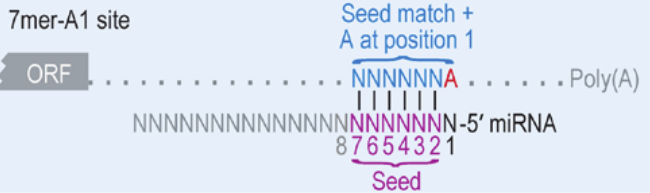
\includegraphics[width=1\textwidth]{microRNA.png}}
	\caption{Schematic representation of the binding of a microRNA on a messenger RNA, for a 7mer site. Illustration taken from \cite{Urich}}
\end{figure}
In that sequence, the most important is the "seed region" (see the figure above for a schematic representation), a complementarity in this region being enough to for the complex to bind the messenger RNA, and most of the time, mandatory. This seed region is located in the 5' region of the microRNA, and could be a 6, 7 or 8mer \cite{site,Urich}. By extension, the seed region is also in the 3' region of the microRNA binding site.

Nonetheless, despite this evidences, the microRNAs' network is still poorly understood \cite{network,cancer}. The reason includes : the functional redundancy of the microRNAs, the lack of clear phenotype when one microRNA is knock-down, the combinational of the repression, etc\cite{network,cancer}. 
Their levels of expression, like many non coding RNA, is altered in disease, including cancer \cite{cancer}.

\section{Inhibition and level of mRNA}

While the description of the mechanism of the translational inhibition above suggest that the levels of microRNA-inhibited mRNAs remain unchanged, more recent work has demonstrated that the repression of many miRNA targets is frequently associated with their destabilization \cite{cancer}.

Micro-array studies of transcript levels in cells and tissues
in which microRNA levels were experimentally altered, revealed marked changes in the abundance of validated or predicted miRNA targets, consistent with an role for miRNAs in mRNA destabilization \cite{cancer}.

\section{MicroRNAs : a paradigm based on cooperativity}

There is experimental evidences for a microRNA cooperativity in the post-transcriptional repression they exert, when their seeds region on the messenger RNA are in close proximity $13\!- \!35$ nt \cite{site, coop}.\\
 Since this could be an effective way to understand how the microRNAs' network exert its repression, a model based on this cooperativity has been tested in sillico. The model predicted the expression level of p21 in 9 of the 12 tissues considered for the simulation \cite{p21}.
\begin{figure}[H]
	\centering
	{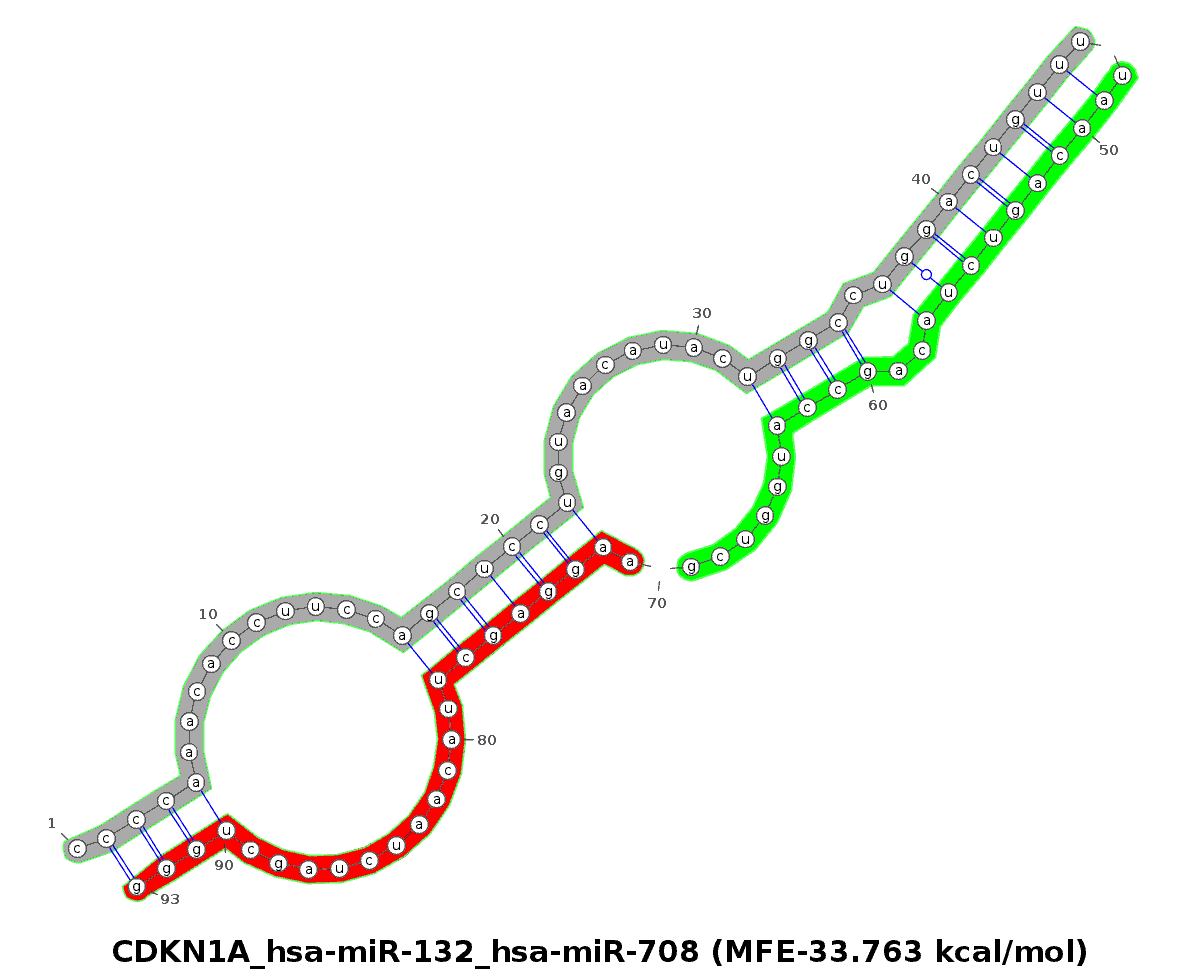
\includegraphics[width=0.8\textwidth]{canonical.png}}
	\caption{An example of canonical triplex, from the triplexRNA database}
\end{figure}

The TriplexRNA database is based on this work. Based on a computational workflow to predict them\cite{triplex}, the database provide putative triplexes, triplexes composed by two microRNAs and their mutual messanger RNA target (three RNA molecules for the triplex, nonobsting the AGO proteins). This report will sometimes refer to this database as the "triplex", for convenience purposes.



\section{Circular RNAs}

Mostly formed by backsplicing\cite{diversity, sponge}, the circular RNA are a class of long non coding RNA.\\
While the exact nature of their function remains elusive \cite{diversity, mir7, sponge}, it has been proved that one of them is to "sponge" the microRNAs\cite{mir7,sponge}. \\
By binding the microRNAs, a circular sponge decoy the microRNAs from their original targets. Since this targets are messenger RNAs, and that the microRNAs exert a repression, the sponge influence the level of expression of the genes regulated by this microRNA, and induce an up-regulation of their traduction \cite{mir7,carcinoma,sponge}.

\begin{figure}[H]
	\centering
	{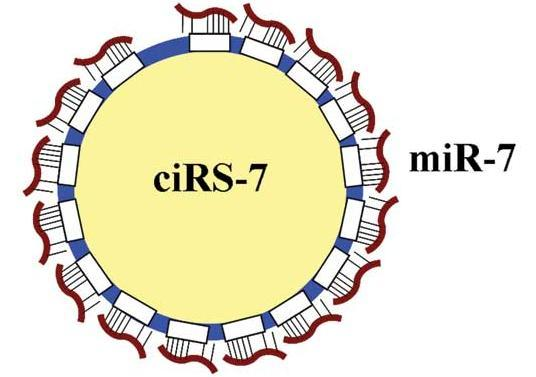
\includegraphics[width=0.5\textwidth]{sponge.jpg}}
	\caption{Illustration of the "sponging" capability of the circular RNAs. Illustration taken from\cite{sponge}}
\end{figure}

This ability to up-regulate the expression of genes, coupled with a long half-life due to their circular shape \cite{sponge}, make them a good candidate as a therapy tools. \\

That could be the case for disease involving a deregulation of microRNAs' level of expression, like in cancer as stated before \cite{cancer}, and their phenotypic consequences in various disease\cite{therapeutics}, or in case the enhancing of traduction of one gene would be suitable.

Some circular RNAs and their absence have also been report to be directly involved in diseases. For example, a circular RNA which sponge miR-9, circMTO1, has been found to be highly  correlated with the prognosis of patient suffering from human hepatocellular carcinoma (HCC) \cite{carcinoma}. Moreover, the circular RNA could suppress HCC progression in vivo\cite{carcinoma}, leading us to think that circular RNAs could be a good therapy tool, once bypassed the usual problems of addressing and delivering of this molecules, common to every RNA therapy\cite{therapeutics}.


\section{Context of the work}

The first objective was to develop an executable which design a circular RNA sponge, to upregulate the level of expression of a gene(s) of interest, using the information contained inside the triplexRNA database. This executable could be then integrated into further release of the triplexRNA. This part was done with success, and this concise report will first show how the executable which design the circular RNA works. The executable which can be found here. The procedure to chooses which microRNAs should be sponge is detailed later in the report.\\

A secondary focus was made on the melanoma cancer.
The main motivation behind this was to extend the previous workflow to upregulate genes of interest, to a workflow to upregulate a pathways of interest.
 Indeed, the triplexRNA can be query for a list of genes and for pathways (the triplex integrate most of the KEGG pathways), including the KEGG melanoma pathways.\\

\section{Why differential expression analysis}

Our goal is to design a workflow to design a circular sponge, to up-regulate a pathways of interest, in the context of a RNA therapy.\\

The triplexRNA integrate such pathways in the form of KEGG pathways, which are a collection of manually drawn pathway maps representing our knowledge on the molecular interaction for various metabolism or disease\cite{KEGG}. And the database actually allow to visualize the mutual "target genes" of a selected pair of microRNA within a KEGG map (the genes being highlighted in yellow on the map).\\

The KEGG pathways are also encode in the base in the form of a list of genes, and by then the triplexRNA database allow to retrieve all the triplexes involving the genes of a pathways, just by selected the KEGG pathways.\\

The problem is : as we want to promote the expression of a pathways in a biological condition of interest, and since the KEGG pathways are only encode as a list of genes inside the triplex RNA, which does not tell us which gene are down-regulated or which are post-transcriptionaly repressed by microRNAs, how to know which genes should have their expression promoted to up-regulate the pathways ?\\




The idea was to find genes differentially expressed between early and late stages of the melanoma cancer, using the Xena database\cite{Xena} to obtain the level of expression of the genes composing the KEGG Melanoma pathway.\\

The choice of the Melanoma cancer have been done because of the potential experimental outcome. For example, the circular RNA sponge could have been tested in cells culture : the experimental design would have been to test if the artificial introduction of the circular RNA would have induced a phenotype reversion of the late stage phenotype toward an early stage phenotype.\\
  
The whole workflow and controls are detailed below, and the limits of such a demarch explored inside the conclusion.


\chapter{Results}
\startcontents[chapters]
\printmyminitoc %print minitoc

\section{First workflow}

Af we stated before, our goal was to investigate the design of a workflow to upregulate a biological pathways of interest with a circular RNA sponge.

Our concern is that KEGG pathways are only implemented as a list of genes involved in disease, inside the triplexRNA database\cite{triplex}, without any further indication on their involvement. We don't know from the base if this genes are down-regulated, up-regulated, or inhibited in the biological conditions of interest. 

A solution is to perform a differential expression analysis on this subset of genes provide by the triplexRNA, to find which genes are lowly expressed in the disease, and potentially responsible of its phenotype.

As we stated in the introduction, the repression exert by microRNA can result in a destabilization of the mRNA target and a change in the level of expression, but this is does not now necessary occur, and microRNA-inhibited mRNAs can have their level unchanged.

Here, we do not presume that the change in level of expression of mRNA is caused by the change in the expression of microRNAs, as it occur in cancer\cite{cancer}, even if it's a possibility. 

We are looking for genes which are potentially responsible for the phenotype. This genes would be then good candidatures to be upregulated or having their expression improved using a circular sponge.

A transversal and complementary approach to the differential expression analysis is a feature selection, operated on the genes.

The feature selection is a field of the machine learning domain\cite{springer}, dedicated to select feature among a set of data, in order to improve the generalization of models, or get a better understanding of the features and their relationship to the response variables\cite{springer}. It is this last aspect which we interest us.

To check the accuracy of such selection, a random forest classifier \cite{springer} has been trained with this set of genes, and the error of classification has been plot.

This approach is still a bit naive, especially regarding the complexity and heterogeneity of cancers\cite{TGCA, complexity}, and the uncertainty behind the causes of the differential expression. For this reason, two control will be perform, one for this two approach.


\begin{figure}[H]
	\centering
	{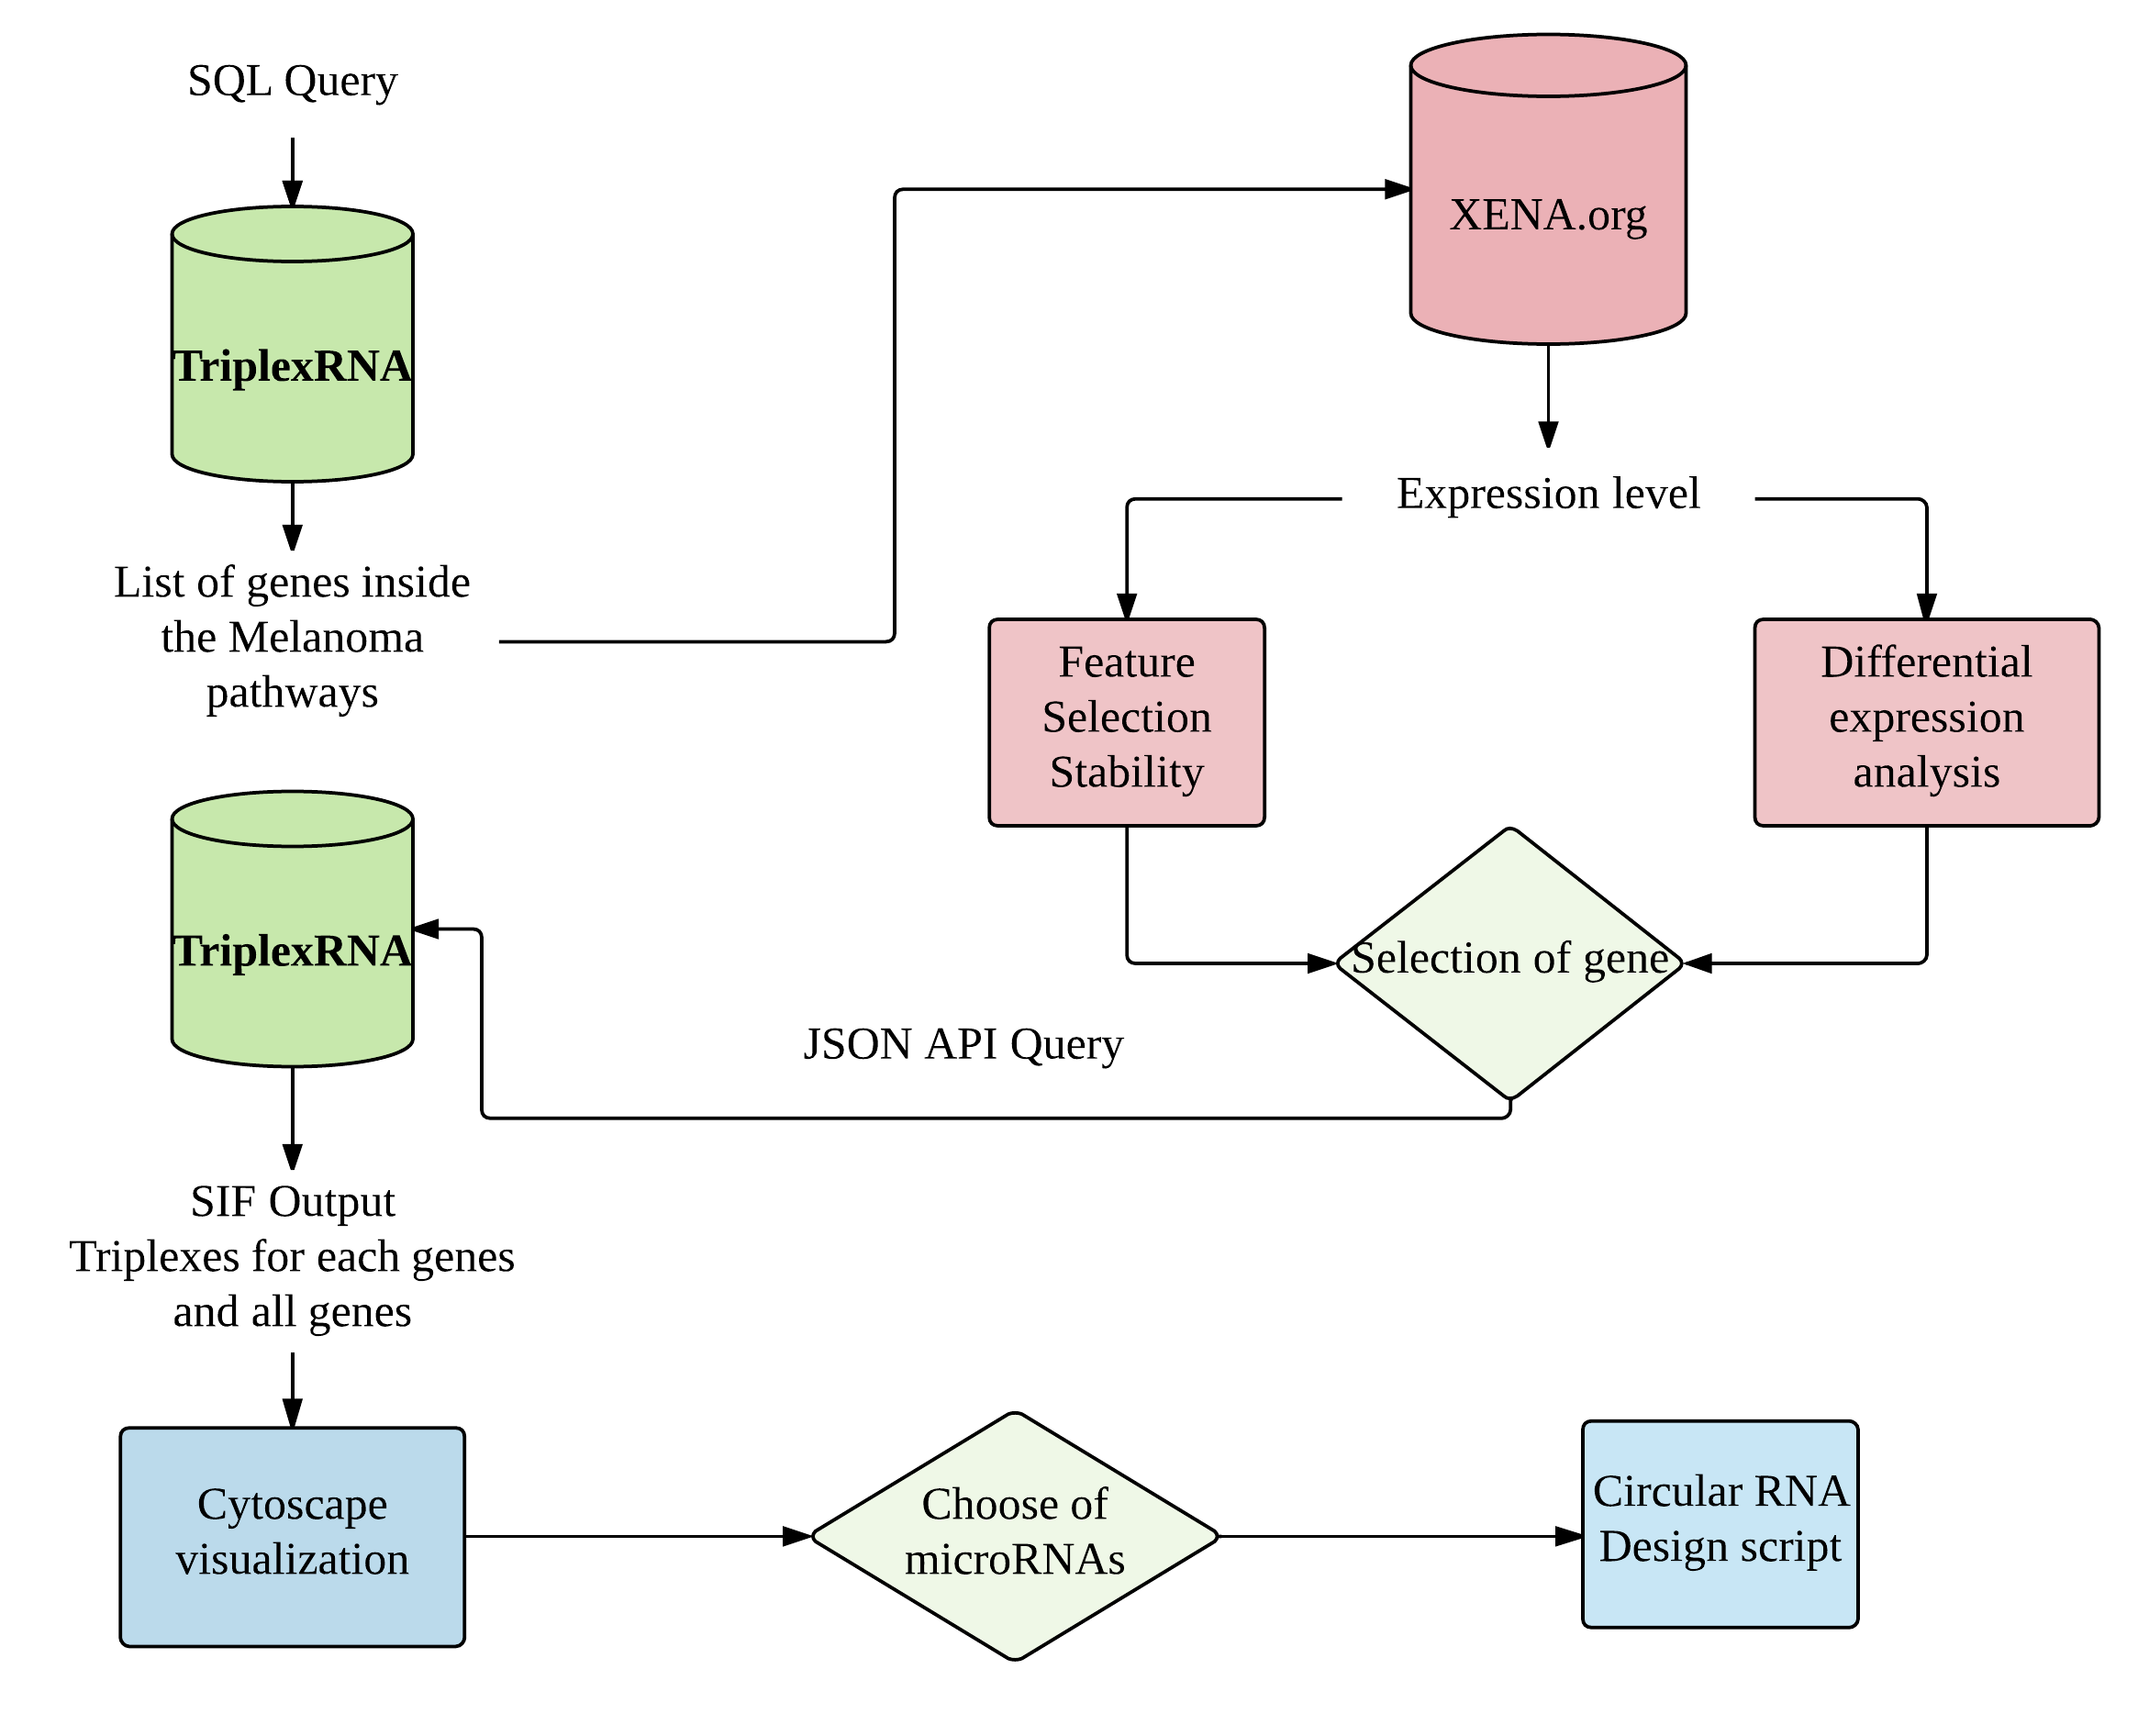
\includegraphics[width=1\textwidth]{Workflow1.png}}
	\caption{The structure of the first workflow. The retrieving of the genes composing the Melanoma KEGG pathways using a SQL query is the first step.}
\end{figure}

\subsection{Differential expression analysis}

The differential expression analysis has been performed using limma \cite{limma}, to find differentially expressed genes between the early and late stage of the melanoma, and then susceptible to be retain as a target for the an RNA therapy with a circular RNA.

As a control, a projection of the sample on a two-dimensional scatterplot, where the distance approximate the expression differences between the samples, has been done.

The plot does not show a perfect separation of tumor from normal samples as expected for a differential expression analysis which performed well (see figure below).


\begin{figure}[H]
	\centering
	\subfloat[Scatterplot where the distance between sample is a projection of the log2 fold change distance, for Melanoma cancer data, between late melanoma and early melanoma.]{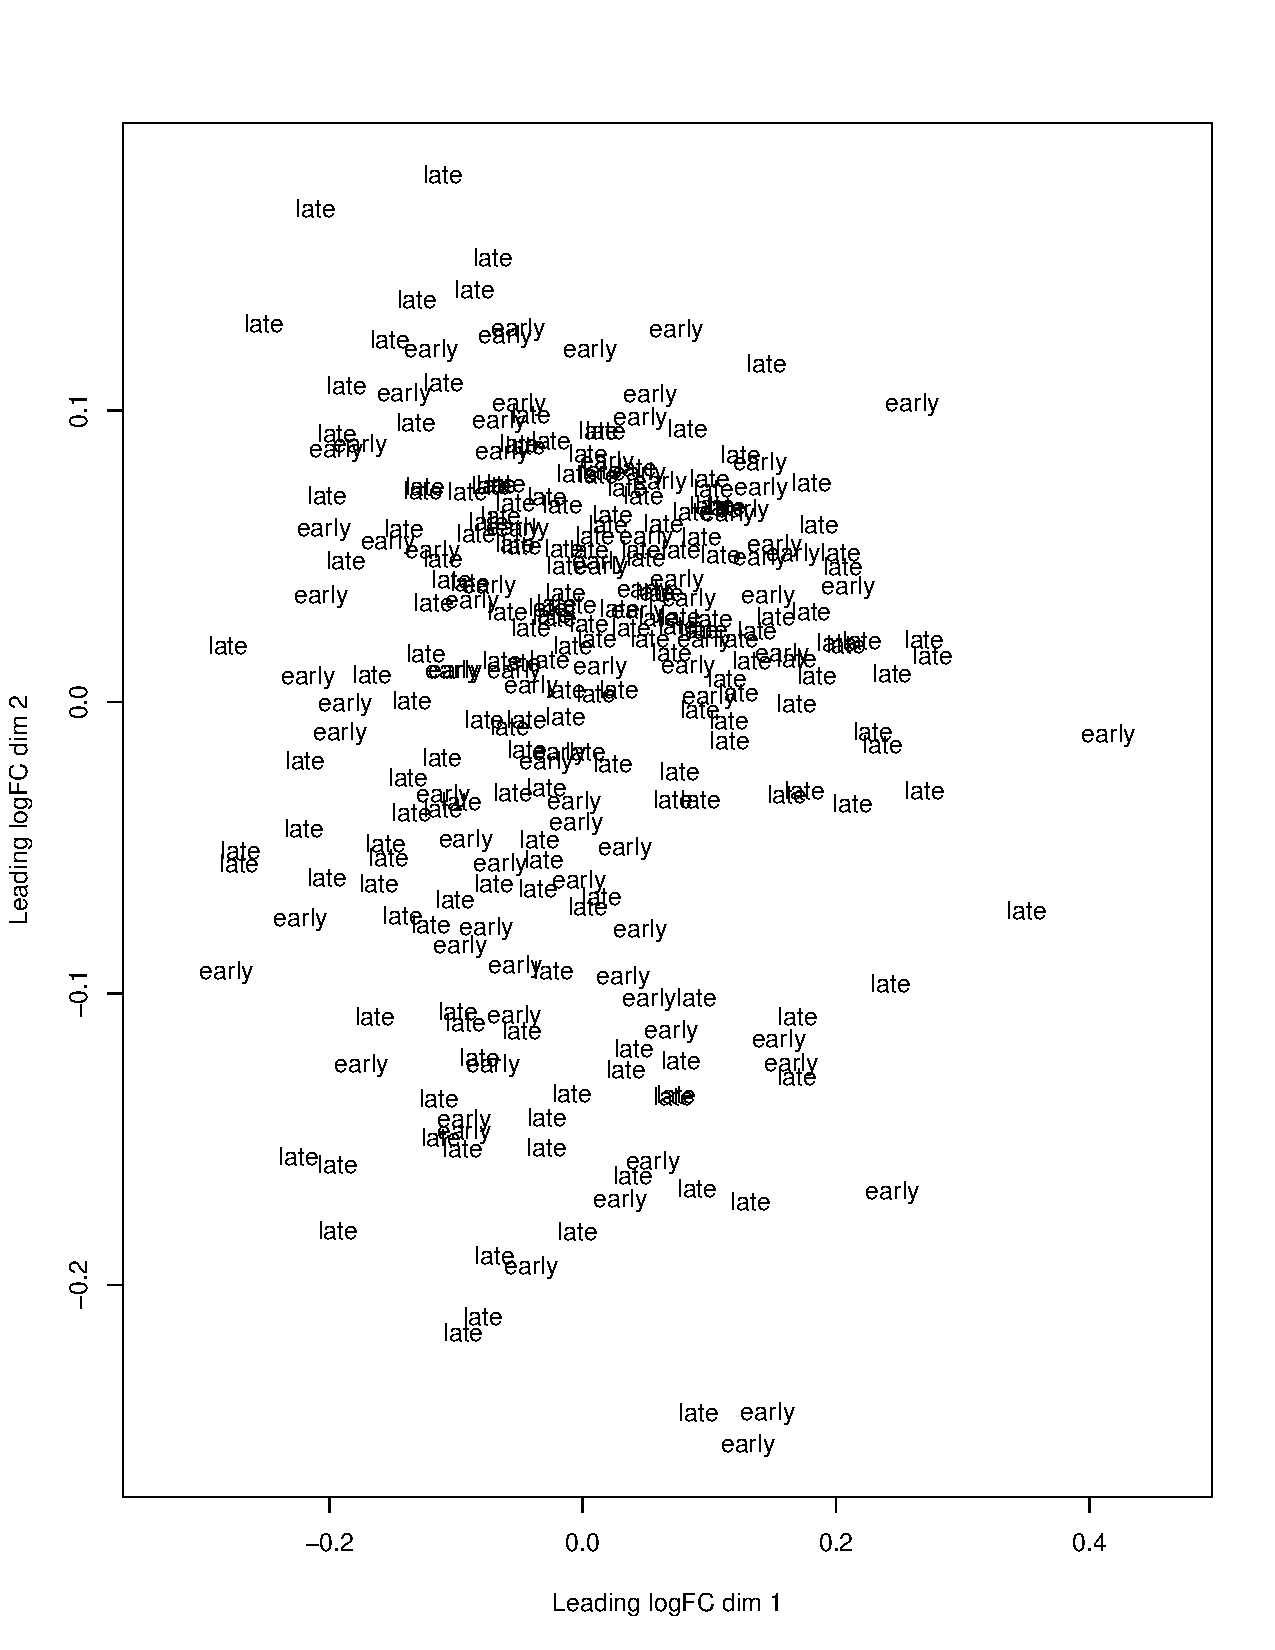
\includegraphics[width=0.49\textwidth]{Rplot_melanoma.pdf}\label{fig:f1}}
	\hfill
	\subfloat[Scatterplot where the distance between sample is a projection of the log2 fold change distance, for Colorectal cancer data, between normal adjacent and cancer cells.]{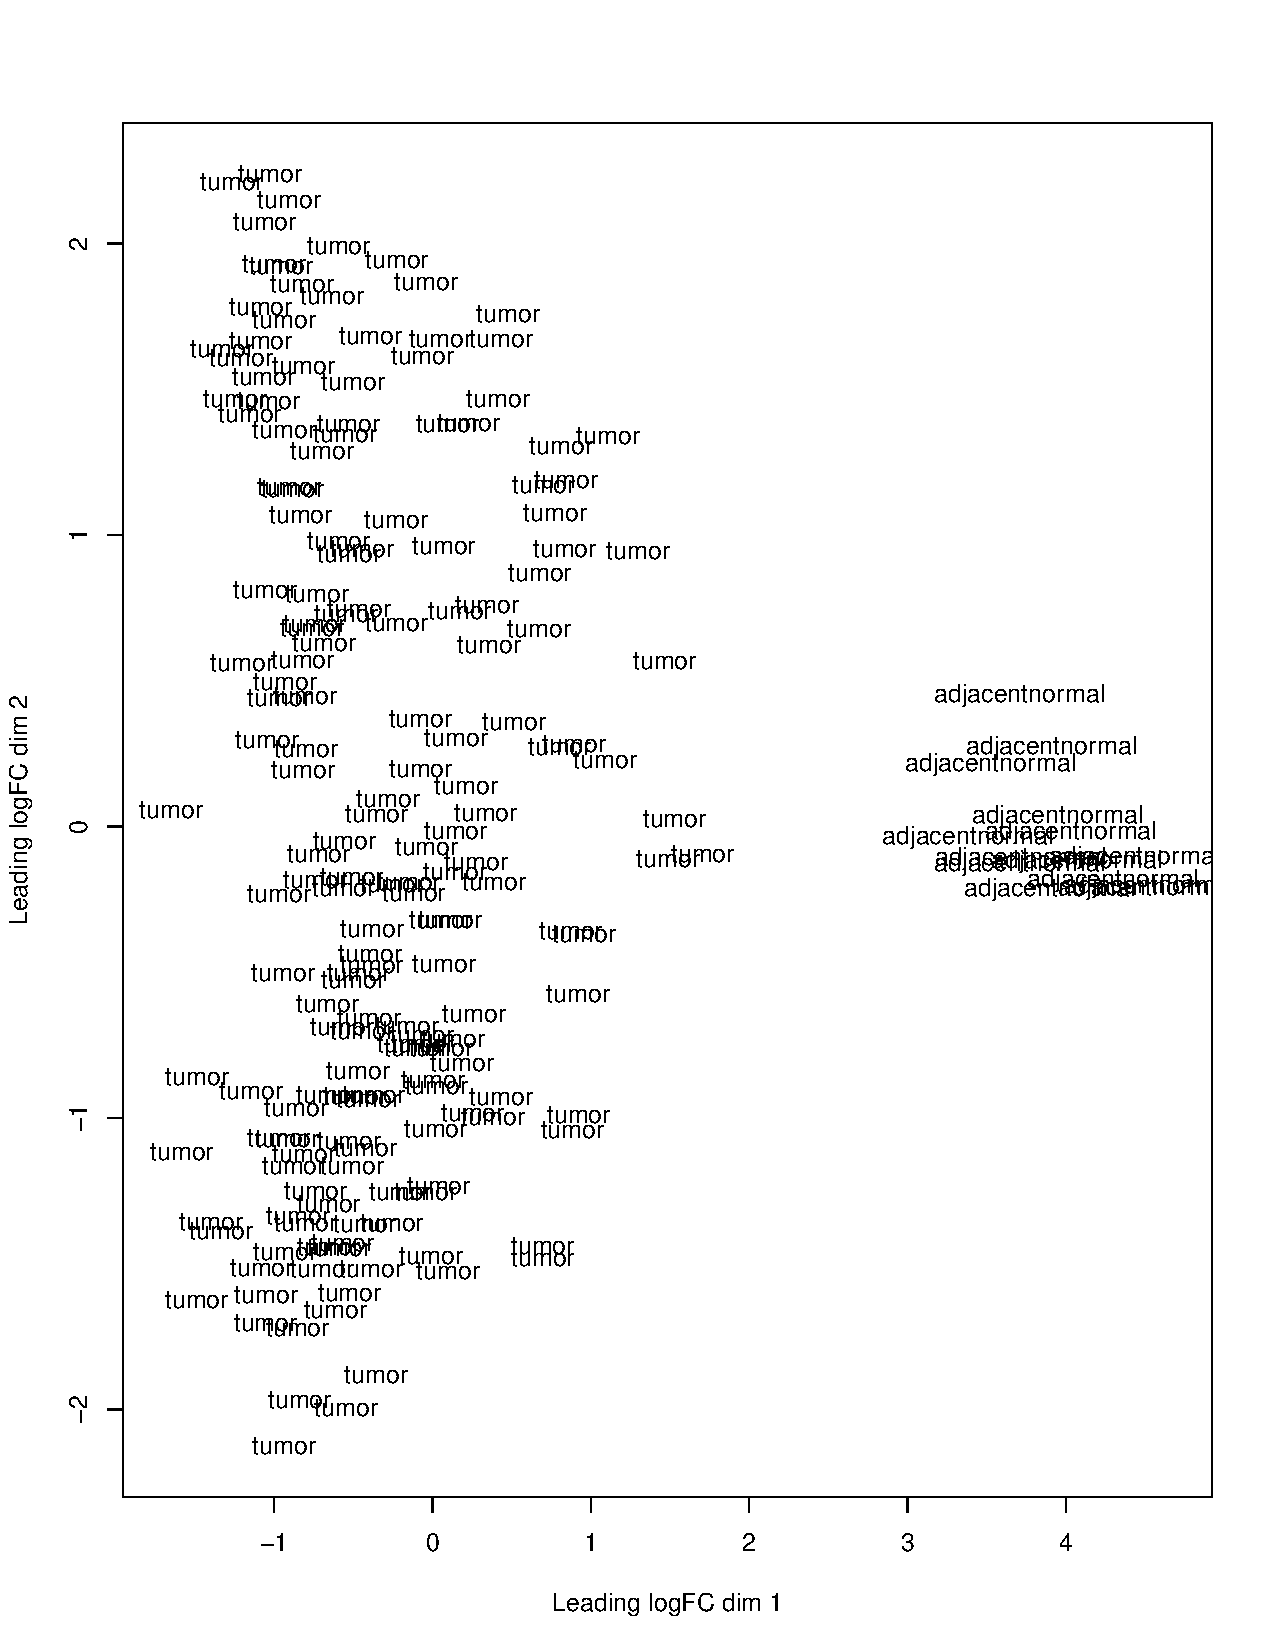
\includegraphics[width=0.49\textwidth]{Rplot_collorectal_cancer.pdf}\label{fig:f2}}
	\caption{Comparison of the projection fold change distance between melanoma sample and colorectal cancer after a differential expression analysis. The scatterplot of the colorectal cancer show the expected output for this analysis, with a good separation of the two groups.}
\end{figure}

\subsection{Feature selection using randomized lasso}

The feature selection method employed was the Stability Selection \cite{stability}, a method based on numerous subsampling of the data set - here, different samples - with different subsets of feature - here, the genes -, in combination with a method of feature selection.

This different subsampling are then aggregated, and a ranking is produced using the features selection method retain. This Stability approach perform well in dataset with a lot of correlation in the data \cite{stability}, assuming that the model is sparse - meaning that only a few genes are responsible for the difference between the two conditions-.

This framework of stability selection has already been used in biology\cite{tigress}, and is implemented for the lasso method inside the scikit learn library\cite{scikit} under the name of RandomizedLasso, a method which has already been deployed to identify cancer driver genes\cite{randomlasso}.

To test this selection of gene, a random forest classifier \cite{springer} has been trained using only this selection of genes as variable, and the error of classification has been plot (see below).

The reason for choosing a random forest classifier is its reliability and the fact that they require less tuning in comparison to other classification method\cite{springer}. This make them ideal to test a selection of genes in a repetitive manner inside a workflow.

Nonetheless, the plotting of the classification error, for the whole melanoma data, but also for subtypes\cite{TGCA} (NRAS, BRAF), did not allow to think that the genes selection was pertinent (cf figure).

\begin{figure}[H]
	\centering
	{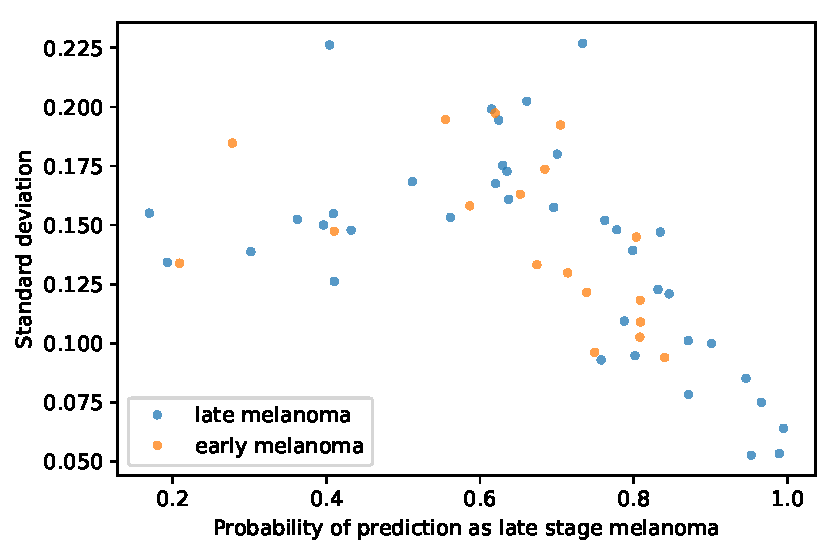
\includegraphics[width=1\textwidth]{forest_prediction}}
	\caption{Error of classification of the random forest classifier, using a selection of genes inside the KEGG melanoma pathways, selection output by the feature selection approach}
\end{figure}


\section{Current workflow}


It appears from the previous section that the use of the KEGG pathways encoded inside the triplexRNA database was not pertinent in the context of choosing the set of genes to run the rest of the workflow.\\

This part of the workflow has been by then edited : the executable which query the script has been edit to retrieve the canonicals triplexes for a list of genes provided as input. For the list of genes, it seems better to rely on the user's expertise to provide it (see conclusion and perspective for more details).\\

To illustrate the current workflow, we will create a sponge in the context of a RNA therapy for the colorectal cancer, using the curated RNA-seq data\cite{curated} used in the previous section to perform the control of the differential expression analysis and of the scatterplot.\\

In order to do so, we will use some of the top genes differentially expressed between the normal condition and the tumor condition.\\

Of course, while this reduced set of genes is sufficient to distinguish between the two condition (see scatterplot with the top12 genes below), they are not necessary responsible for the differences in the phenotype between the normal adjacent cell and the tumor cells, and promoting the expression of genes down-regulated in the cancerous cells will not necessary end in a reversion of the phenotype of the cancerous cells into normal cells (see conclusion for further details and discussions).\\

Such a diagnostic would require more investigation, using ontologies and literature for that cancer\cite{colorectal}. Here we select this genes for illustration purpose. A normal use of the workflow would rely on the expertise of the user and that the user provide a set of genes for which he want to promote the expression.\\

\subsection{Diffential expression analysis, Colorectal Cancer}

\begin{figure}[H]
	\centering
	\subfloat[Projection of the fold change between normal cells and tumor cells for colorectal cancer.
	]{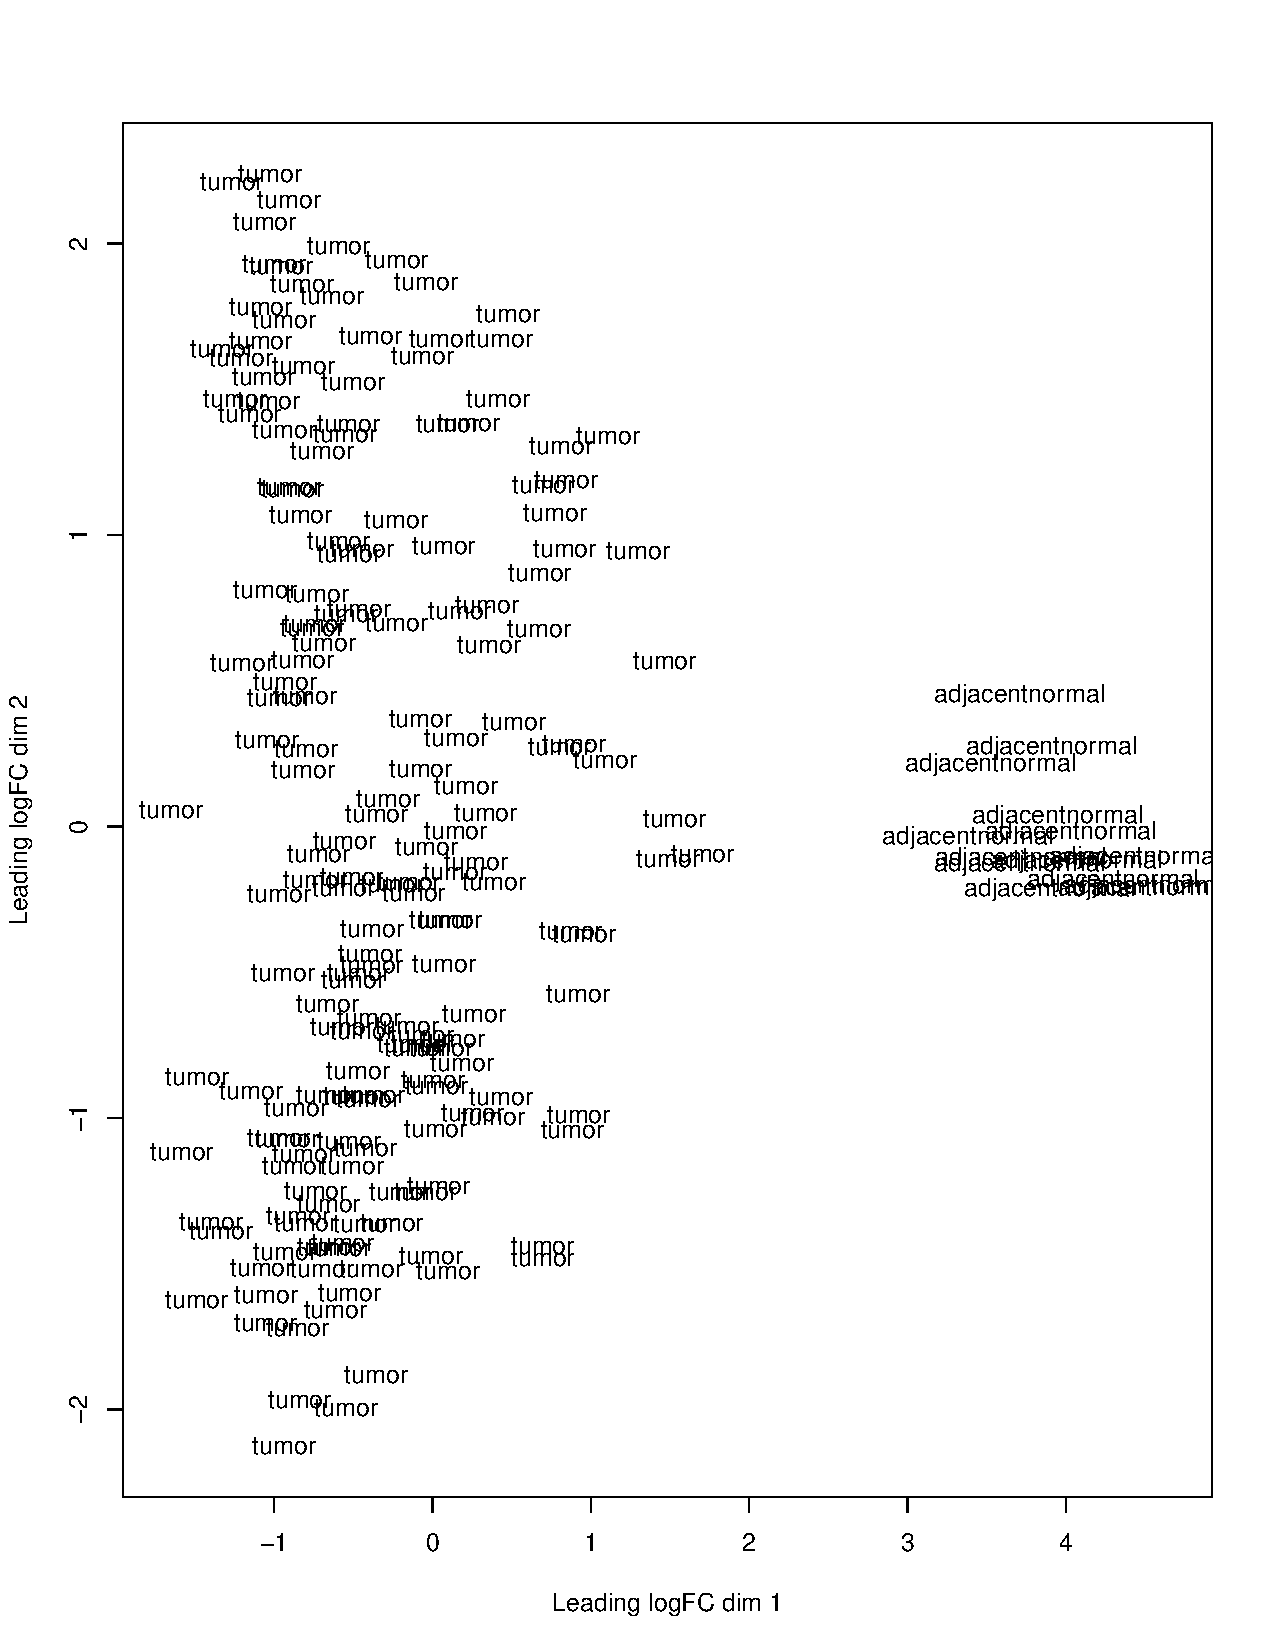
\includegraphics[width=0.49\textwidth]{Rplot_collorectal_cancer.pdf}\label{fig:f1}}
	\hfill	
	\subfloat[Projection of the fold change between normal cells and tumor cells for colorectal cancer, using only the top 12 of the differentially expressed  genes.]{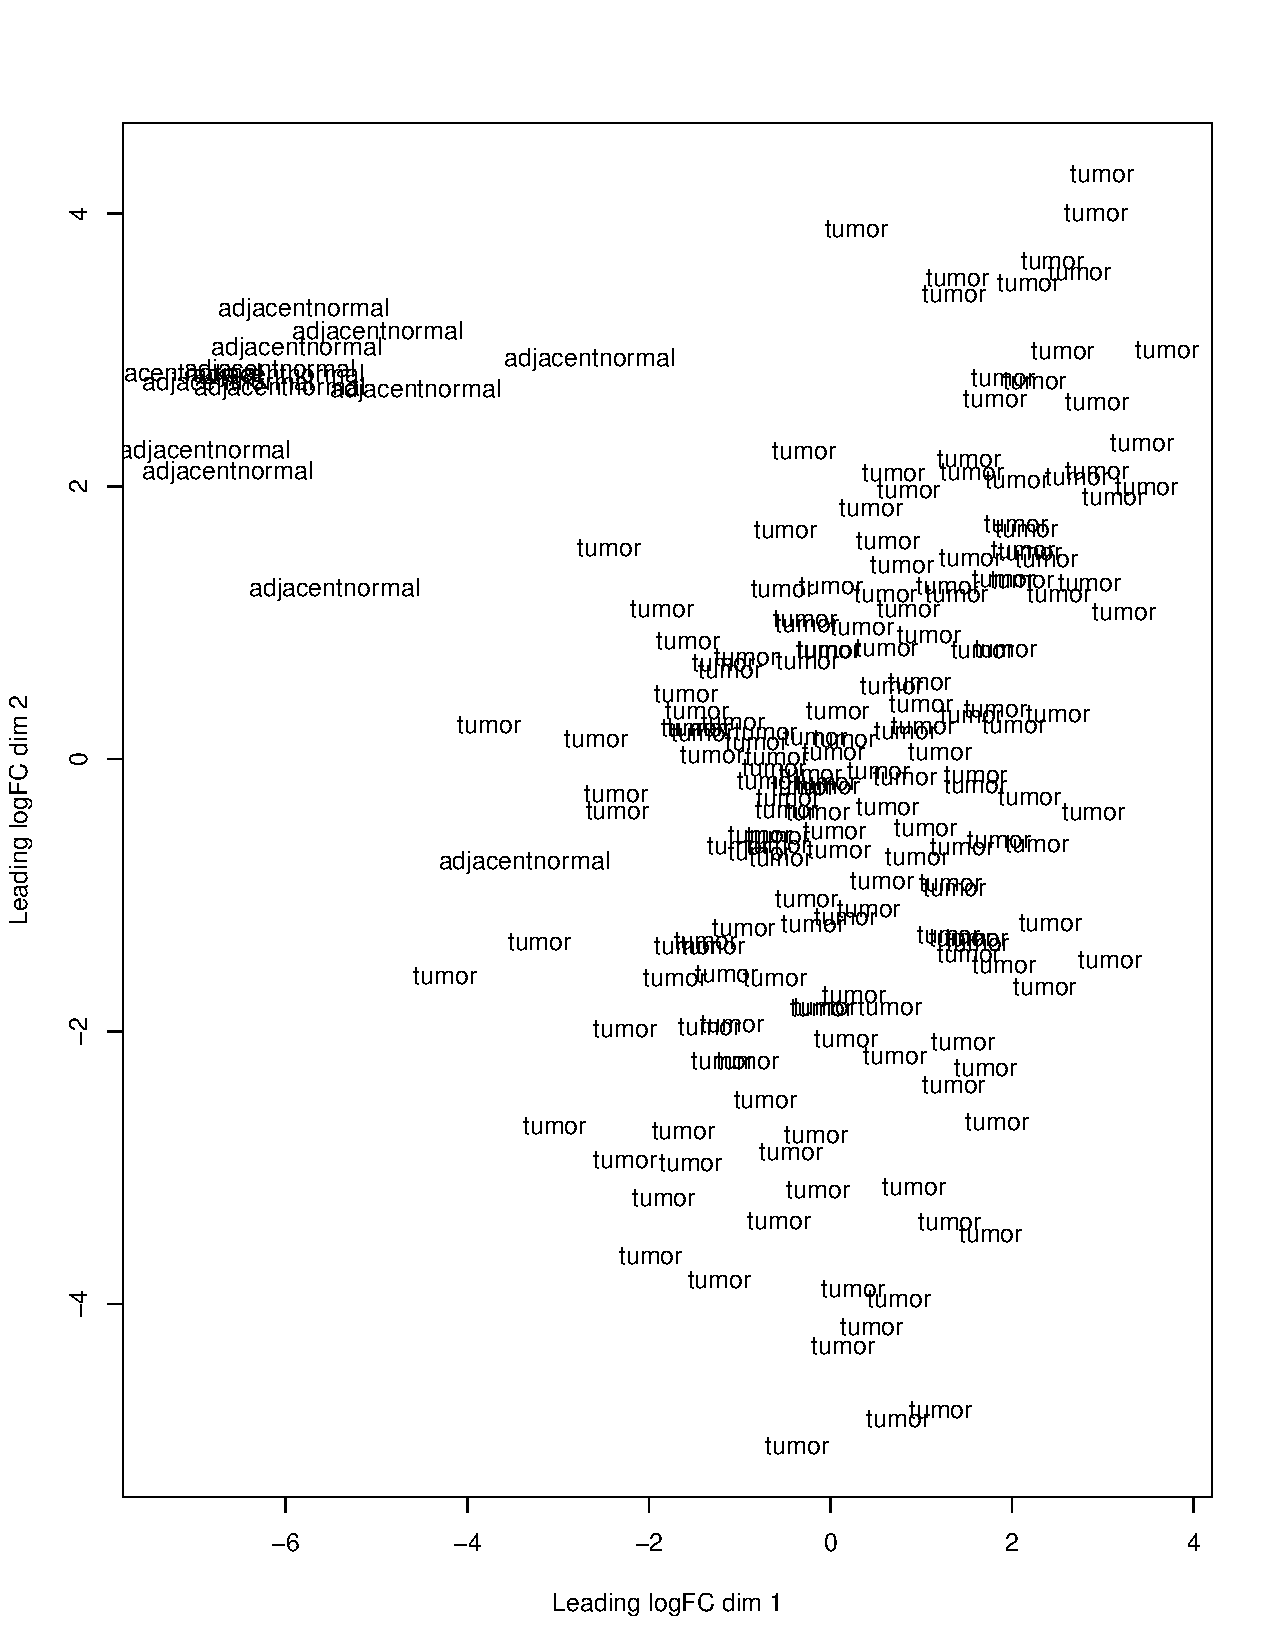
\includegraphics[width=0.49\textwidth]{Rplot_12_genes.pdf}\label{fig:f2}}
	
	\caption{Multidimensional scaling plot of distances, using the plotMDS() function from edgeR. In the context of using a reduced number of genes to distinguish between the two conditions (normal adjacent cells and cancerous cells), we observe a good separation with the top 12 of the differentially expressed genes.}
	
\end{figure}

\subsection{An executable to query the triplexRNA}

The executable which was used to retrieved the list of genes inside a pathways, and the canonical triplexes for this genes, was modified to retrieve the canonical triplexes for a list of genes past as input in a text file.\\

The script retrieve all the triplexes involving this genes, using a JSON query for each genes from the list of genes (see material and method), with a filtering of the redundant triplexes (see below and the material and method), to avoid any bias in the estimation of the importance of some microRNAs, and keep only the canonical triplexes, which are the functional triplexes according to the workflow publish by Schmitz et al.\cite{triplex}.\\

Redundant triplexes are triplexes in which the two microRNAs bind the messenger RNA at the same positions, with one microRNA in common among all the different triplexes.\\

This redundancy phenomenon appear when one particular microRNA form nearly identical canonicals triplexes with all the member of a microRNA family, since microRNAs from the same family can arbor nearly identical sequences except for some nucleotides outside the seed region.\\

While this triplexes are different biochemical entities, they can not cumulate their repression on the same molecule of messenger RNA, since the microRNAs of this redundant triplexes bound the messenger RNA on the same place.\\

This introduce a bias in the following steps of the worfklow when we aim to find which microRNAs have the most partners. A microRNAs involved in several redundant triplexes will be seen as with multiples partners, while its sponging will only remove the repression of one pair of cooperatives microRNAs on the same molecule of messenger RNA.\\

This executable, which query both the web instance of the triplexRNA and a local instance of it, ouput a sif file format. This sif file contain all the canonical triplexes for the list of genes (see material and methods), and is meant to be used as input for the software Cytoscape \cite{cytoscape}, the following set of the worflow.


\subsection{Cytoscape visualization}

The outputted file by the script which retrieve all the triplexes for a list of genes is in a sif format, and can be passed as input to the software Cytoscape\cite{cytoscape}.\\

Cytoscape is an open source software platform for visualizing networks. While it can seem a curious choice when it comes to microRNAs, this transformation of data in the form of a non oriented network, where the edges are the triplex ID and the nodes the microRNAs, allow to visualize which microRNA form a pair with which microRNA, and to identified easily which microRNA has the most partners.\\

In other words, this allow to retrieve which microRNA should be sponge to remove the most triplexes and promote the genes expression.\\

This format specifies only nodes and interactions and it is written as follow :\\


nodeA relationship\_type nodeB 

nodeC relationship\_type nodeA \\


Also, while the sif file format specify only nodes and interactions, the software Cytoscape merge by himself the nodes with the same names. This allow to require only a simple format as output for the previous script, to retrieve all the triplexes.\\

So, Cytoscape allow the user to visualize the pair of cooperative microRNAs which exert a repression on the genes passed as arguments, under the form of a network (cf figure). This transformation of the data is meant to allow an easy visualization of the relative importances of each microRNAs.\\

MicroRNAs which have the most partners, and by then those for which the sponging with a circular RNA will remove most of the pairs of collaborative microRNAs can be identified by looking at the nodes with the more edges.\\

The user can then provide this names as input to the next step of the workflow, the circular design script.\\


\begin{figure}[H]
	\centering
	{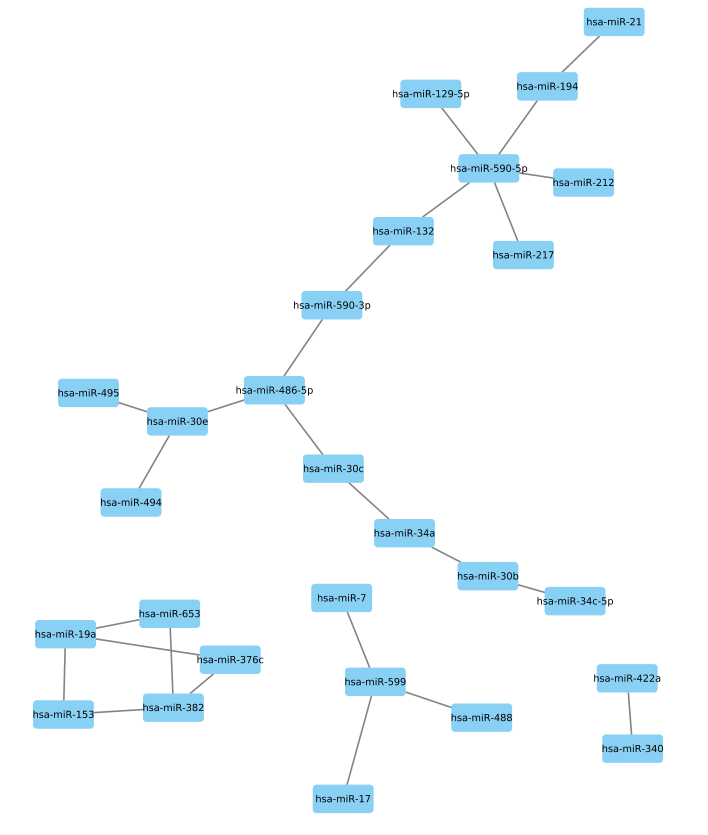
\includegraphics[width=1\textwidth]{cytoscape_output.png}}
	\caption{The Cytoscape visualization for 3 downregulated gene in colorectal cancer, comparde to normal adjacent cells. This genes are BEST4 (4 triplexes), LGI1 (20 triplexes), KRT24 (14 triplexes). Here hsa-miR-590-5p is a potent input for the circular RNA design script.}
\end{figure}

\subsection{Circular RNA design script}

The circular RNA design script is write in Python, is executed in command line, and take as argument, not genes names, but the microRNAs' names that the sponge should decoy from theirs original target. The procedure to choose which microRNAs to sponge is detailed later.\\

More precisly, the circular RNA design script have to mandatory input :
\begin{itemize}
	\item a file  contening the names of the microRNAs that the user want the sponge to decoy from their original target. The names have to be the same than the one in the triplexRNA database. This file is a txt file with just the name of the microRNAs, one per line.
	\item a file containing a priorities for each microRNAs. Basically, the script build the sponge in a recursive way, and add as many binding site as the priority number allocated to each microRNA on each recursion. For example, for a sponge with twice the number of binding site for one microRNAs compare to the other, the file will contain the integer 2 and 1. This file is a txt file with just one integer per line, and have to be in the same order than the microRNAs they refer to.
	
\end{itemize}

The script will then query the triplexRNA database, using the provided names to get the mimat IDs which identify this microRNA in the database. This ID is then used to query Mirbase, to get the sequence of the microRNA. \\

There is several reasons to this. First of all, while the sequences of the microRNAs are encode inside the triplexRNA database, the orientation of the strand is not indicate (5' and 3' extremity), and this step is then a security control, assuring the sequence of the microRNA is in the right orientation.\\

Also, the name of some microRNAs can be different between Mirbase and the triplexRNA, depending on their respective update. For example, most of the microRNAs have the mention 5p or 3p in their name, indicating from which part of the hairpin they come from, a mention sometimes absent from the name inside the triplexRNA database. This step is then a disambiguation phase. 



\begin{figure}[H]
	\centering
	{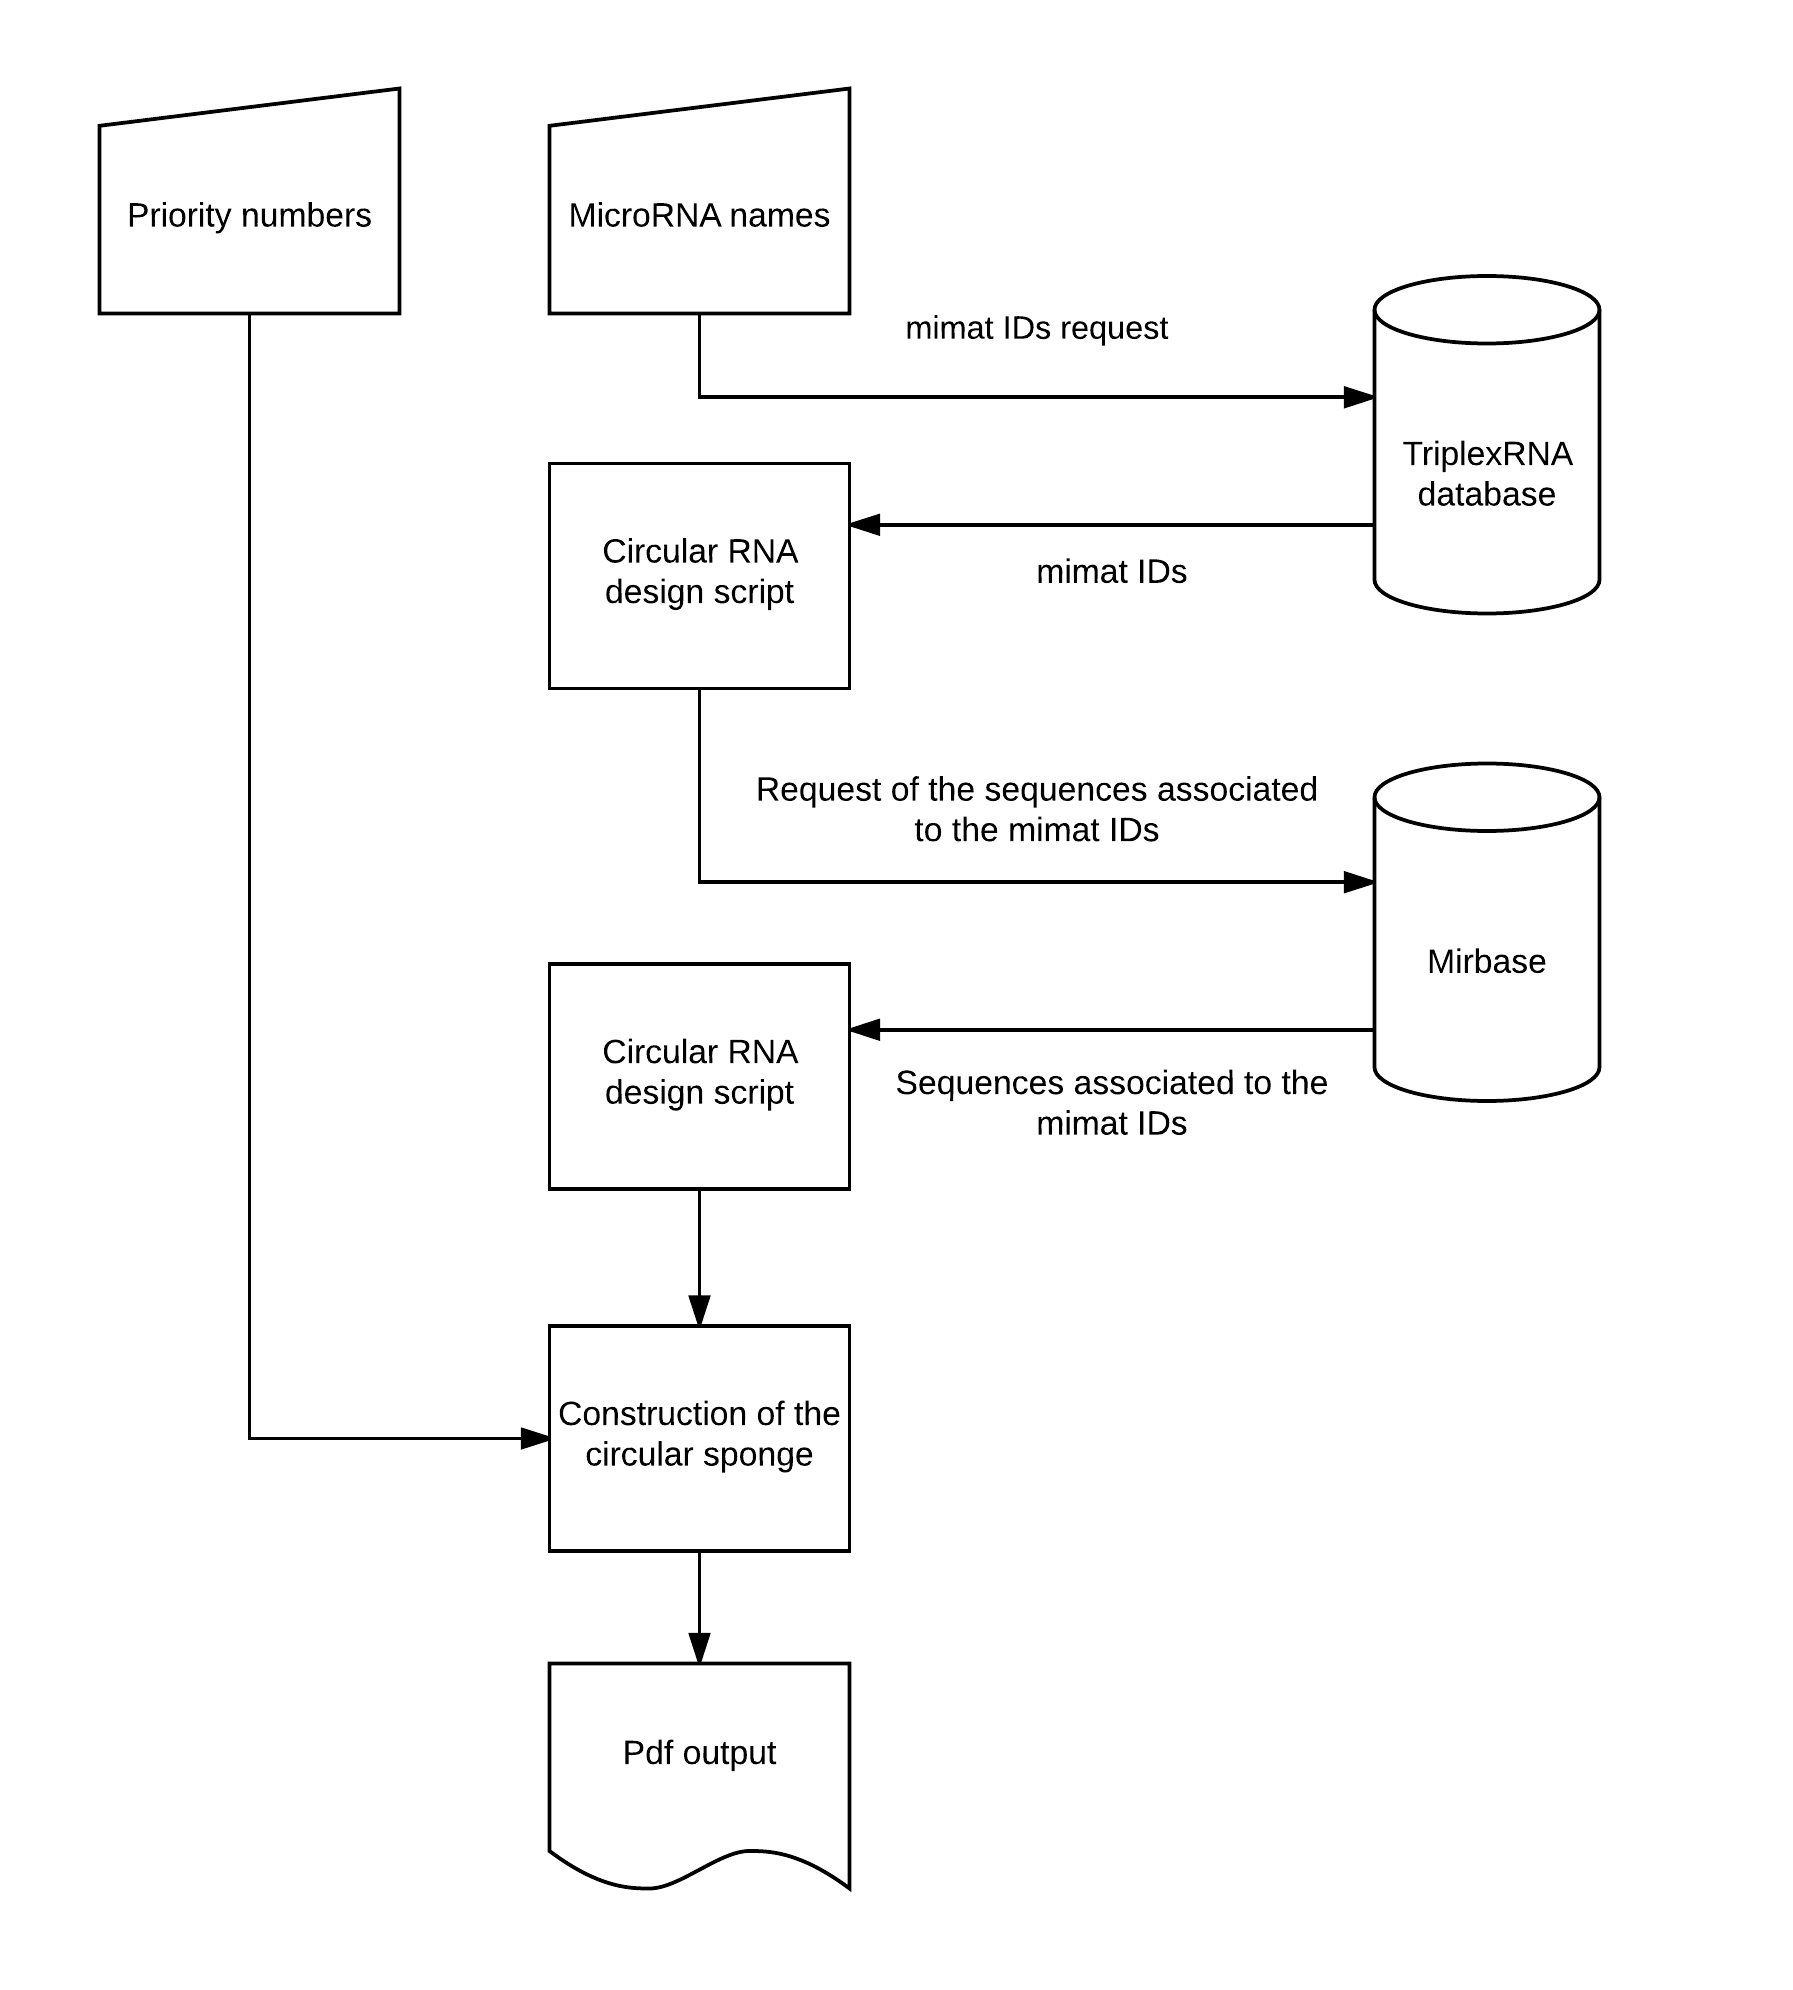
\includegraphics[width=1\textwidth]{Blank.png}}
	\caption{Details of the request done by the circular RNA design script.}
\end{figure}

Once the sequences of the microRNAs are obtain by the circular design script, it will use them to build the most efficient binding site possible for each of the microRNAs. Those building sites, one per microRNAs, will be then repeat on the circular sponge, separated by nucleotides according to another parameter, the distance of cooperativity\cite{coop}. \\

In order to do so, the design script is implemented with rules extract from the scientific literature :

\begin{itemize}
	\item a A is systematically put in first position (in 5') of the microRNA's binding site. There is an overrepresentation of conserved adenosines flanking the seed complementary sites\cite{Aanchor}, among other data suggesting that a site with a A in first position outperform the others one, including the one with a complementary nucleotide to the microRNAs\cite{Urich}. 
	
	\item the seed region (from the 2nd to the 8th nt, cf introduction) is build by inserting complementary nucleotides to the microRNAs' ones, forming a "8-mer" site. See \cite{Urich, site} for further details and representation.
	
	\item a A is put in the ninth position of the binding site, because there is an overrepresentation of conserved adenosines flanking the seed complementary sites\cite{Aanchor}, and because the microRNAs binding sites which perform the best are the ones with a local hight content of Adenine (A) and Uracile (U), over any other variable or predicator \cite{Urich}.
	
	\item the 12th from 10th nucleotides are not complementary to the microRNAs', and U and A if possible. The aim is to avoid any Ago2 mediated cleavage of the circular RNA, cleavage which occur in case of near perfect complementarity between the microRNA sequence and the binding site \cite{cancer}. This nucleotide are U, or A if not possible.
	
	\item the nucleotides from 13 to 16 (included, so four in total) are complementary to the \-microRNAs' one. The reason is that Watson-Crick pairing to four contiguous nucleotides produce an additionnal pairing in 3'\cite{site} and that most downregulation is associated to this additionnal pairing if it start at the 13th position \cite{site}, additionnal downregulation which can be translate as a stronger binding of the microRNA on the binding site\cite{site}.
	
\end{itemize}

As we just mentionned, the microRNAs binding sites which perform the best are the ones with a local hight content of A and U, over any other variable or predicator \cite{Urich}. \\
This is probably correlated to binding site accessibility, and a low potential of forming a self-interacting secondary structure \cite{Urich}. \\
To take advantage of this two features, in order to improve the efficiency of the circular RNA sponge, the script design the sponge's sequence with as many U and A as possible. \\ 
That means that, outside the seed region, where a strict complementarity is required, or in the additional 3' pairing region (cf above), the sequence is write with U or A. \\ A cognate problem is that some proteins target and bind some AU rich sequences, known as AREs \cite{AREs}. However, since this AREs sequences contain some A \cite{AREs}, the safest option is to specify a U prior to an A when writing the sponge's sequence, when no other specific nucleotides is required for complementarity between the sponge and the microRNA. \\

Each binding site is terminated by an additional number of nucleotides, in order to separate its seed from the seed of the following binding site by the distance of cooperativity, as define in \cite{coop}. The distance of cooperativity is the distance between the two seed, distance which insure that the two microRNAs will coopere to bind and exert their translational repression on a messenger RNA \cite{coop}.\\
The distance of cooperativity is set by default to 17, but can be specified by an additional parameters when running the script.\\

The binding sites for one microRNA are organized in cluster by the design script, considering the observation that Ago2 shuttles between adjacent target and then that neighboring sites could cooperate to retain the Ago2-miRNA complex.\cite{cluster}. \\

During the recursive call, the design script build the clusters by adding as many binding site to the cluster as the priority number allocated to this microRNA. The recursive call is interrupt when the limit size (set by default to 300, but can be specified), is about to be exceeded by the addition of a new binding site.\\


\begin{figure}[H]
	\centering
	{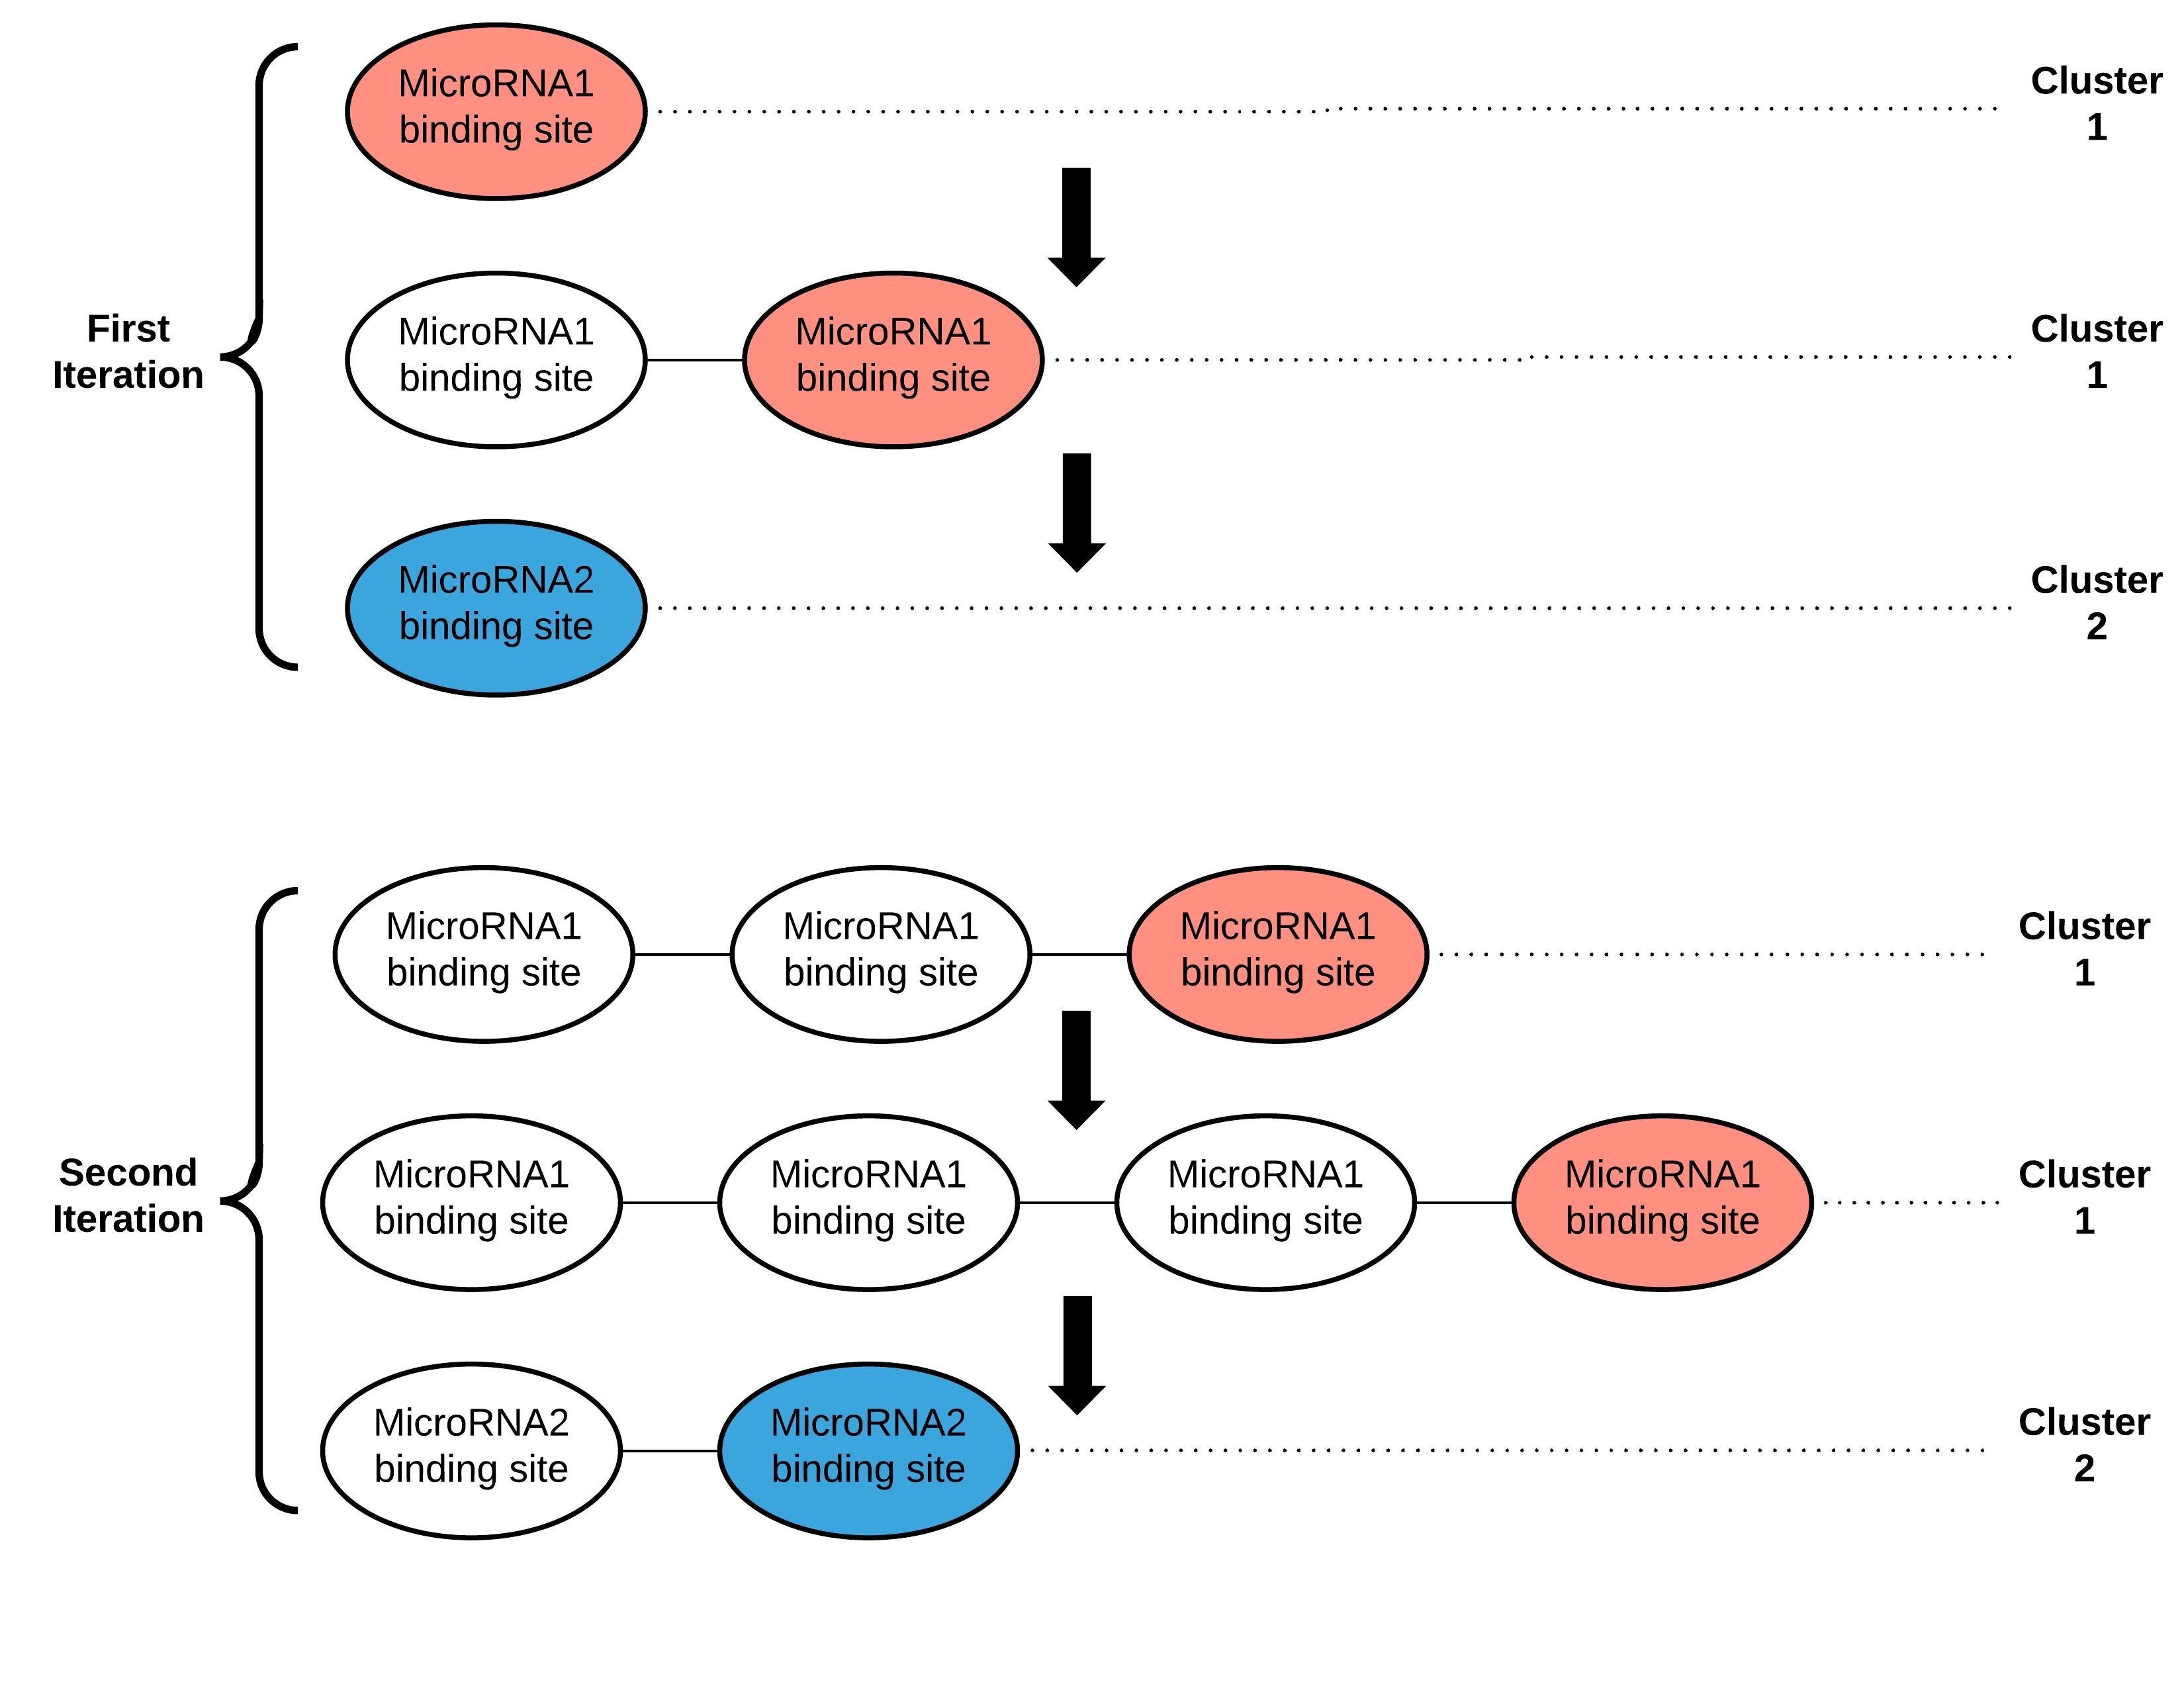
\includegraphics[width=1\textwidth]{circular1(1).jpeg}}
	\caption{Schema of the circular RNA's construction. During the recursive call, the function add on each cluster of microRNA' binding site, as many binding site as the priority number for this microRNA, until the limit size is about to be exceeded. Please take note that the addition of the binding sites is done in a iterative way.}
\end{figure}


After this, the design script compute the minimum free energy of the circular RNA for every arrangement of clusters of binding sites in the sequence, and select the sequence of the circular RNA with the lowest minimum free energy for the output. \\



Finaly, a pdf report with the sequence of the circular sponge is output by the design script. This pdf report details and justifies every step of the design to the user (organization of the binding site in cluster, the design rich in U, etc).\\
This pdf report also provide quality controls in the form of miranda alignments. In this section are exposed the 3 best alignments (if they exists) for each cluster against every human microRNAs. The script is provide with the file mature.fa, a fasta format sequences of all mature miRNA sequences, download from miRbase in may 2017.\\

Each alignments have for title the name of the microRNA performing the alignment, and the name of the microRNA for which the cluster has been design. \\
\begin{figure}[H]
	\centering
	{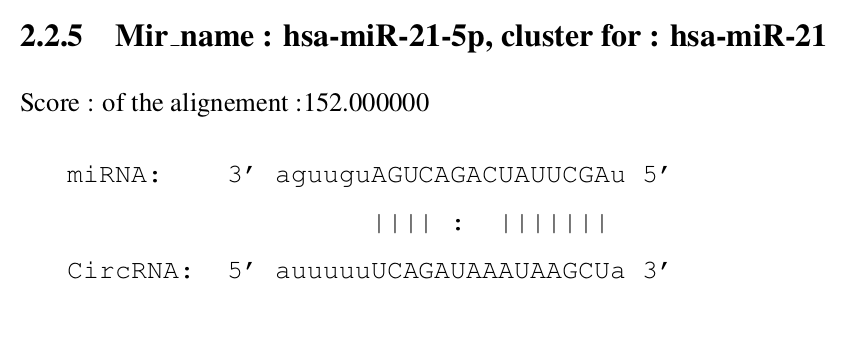
\includegraphics[width=0.8\textwidth]{Capture.png}}
	\caption{Example of one of the alignment found in the pdf report.}
\end{figure}

This allow to check easily if the best alignment is performed by the microRNAs for which the binding site was created, and make sure that the binding site will not be bound by another microRNAs. Or even worse, to ensure that no microRNA is susceptible to trigger a Ago2 mediated cleavage of the sponge.\\

In such case, an override procedure is implement. Providing a txt file with a sequence, the user can redo the whole design process with a binding sequence specified for one or more microRNAs. The construction of the circular sponge is then redo in the same recursive way, except for the creation of the specified binding site, and then the quality control are reperformed and a pdf report is recreated. 


Since all the quality control are performed again, this allow the user to refine the construction of the sponge, especially in the case of one miss design, as describe above.\\

Most of the case of competition by another microRNA are due to a U:G wobble, an allowance between a G in the microRNA's sequence and a U in the sequence of the circular RNA (there is a good example in the figure 2.3), the probability of such an event beeing incredibly improved by the design rich in U of the sponge.\\

In that case the pdf output advise to first replace this problematic U by a A, if possible, to keep the low probability of the binding site to form a self secondary structure.\\
















\chapter{Conclusion and Perspectives}
\startcontents[chapters]
\printmyminitoc %print minitoc

\section{Outcomes}

\subsection{Circular design script}

The major outcome are the two executables which can be found at the following url : https://github.com/Cdk29.\\

While one is only a local API to query a local instance of the triplexRNA, the other one can be used by anyone and independently from the workflow.\\

The circular design script automatize the construction of a circular RNA to decoy particular microRNAs. It takes as mandatory input a file with the names of the microRNAs which should be decoy, which ease any repetition of the process, and a file with priority numbers. This numbers are an intuitive way to create a circular sponge against several microRNAs without allocating to them the same space on the sequence of the circular RNA. Finally the script retain the circular sponge with the minimum free energy.\\

For the construction of the circular sponge, the user can also specify the maximum size for the circular RNA, a distance of cooperativity between the seed, as define in Saetrom et al\cite{coop}. \\

The script finally compile a latex file online using the web tool TEXPILE. The pdf file obtained in this way contain the sequence of the circular RNA, a justification of the design of its characteristics, and the results of alignments perform against all the mature human microRNAs, using miRanda. This construction can be refine and redo by specifying a particular sequence for the binding site of one or several microRNA. \\

While this script can be used separately from the triplexRNA, it's require that the user use the same names as the ones inside the triplexRNA database\cite{triplex}. 

The code of the circular design script is hosted on Github :\\ https://github.com/Cdk29/circular\_RNA\_design where an example of the pdf report is provided.

\subsection{Workflow structure}

The differential expression analysis and the feature selection performed in the first workflow was a tentative to take advantage of the fact that KEGG pathways are encoded inside the triplexRNA database and to have a list of genes of interest.\\

Since this approach was not concluding, it has been removed, leaving us with a workflow without any process to select the list of genes.\\

The form retain for the worflow rely on the user to provide the genes of interest, as it seems more favorable to rely on the user's expertise (see below).\\ 

To retake the exemple of Hepatocellular Carcinoma (HCC), which is develop in the introduction and in this chapter (section below, cirMOT1 in hepatocellular carcinoma), not all the genes differentially expressed in the Hepatocellular Carcinoma cancer are responsible for the invasive phenotype\cite{example}, some being responsible for the migration, immune escape, etc\cite{example}.

A circular sponge designed against the microRNAs involved in the most triplexes involving the messenger RNA of the top down-regulated genes in the HCC may not have been as effective as a sponge targeting specifically the microRNAs targeting the mRNA CDKN1A or a sponge designed against mir-9. \\

For this reasons, and the fact that levels of microRNA-inhibited messenger RNAs may remain unchanged (see subsection "Down-regulation ad translational inhibition below) the structure of the workflow retained rely on the user's expertise, which provide the list of genes to start the workflow.\\

\subsection{Workflow}

The workflow retrieve all triplexes which are predicted to be functional according to the workflow published by Schmitz et Al \cite{triplex}, for a list of genes passed as input of the query script.\\

The workflow provide then a output file for a graphical visualization of the cooperation between the microRNAs which exert a post-transcriptionnal repression of the genes inside the list, using Cytoscape\cite{cytoscape}.\\

That way the workflow provide a tool to visualize which microRNAs are involved in the most pairs of cooperative microRNAs and by then which microRNA to sponge with the circular RNA to affect the most pairs and relieve the most of the repression exert on the list of genes passed as input.\\

The workflow finally provide a design script to automatize the construction of a circular RNA to decoy this microRNAs, providing a pdf report justifying the key points of the design and providing quality control in the form of alignments, using miRanda.\\

The design script allow the user to specify parameters : the list of microRNAs to be decoyed, a list of priority which is an intuitive way to prioritize the sponging of some microRNAs, and a maximum size according to the user synthesis facilities. The size distance between the seed can be specified to adapt to new scientific evidence.\\

Finally, the script allow to refine the design of the circular RNA sponge, through a repetition of execution of the design script. Since the alignments are perform again, and that the microRNA binding site sequence can be specified manually, the user can adjust the sequence of the binding sites according to the results of the alignments on every steps.\\

\begin{figure}[H]
	\centering
	{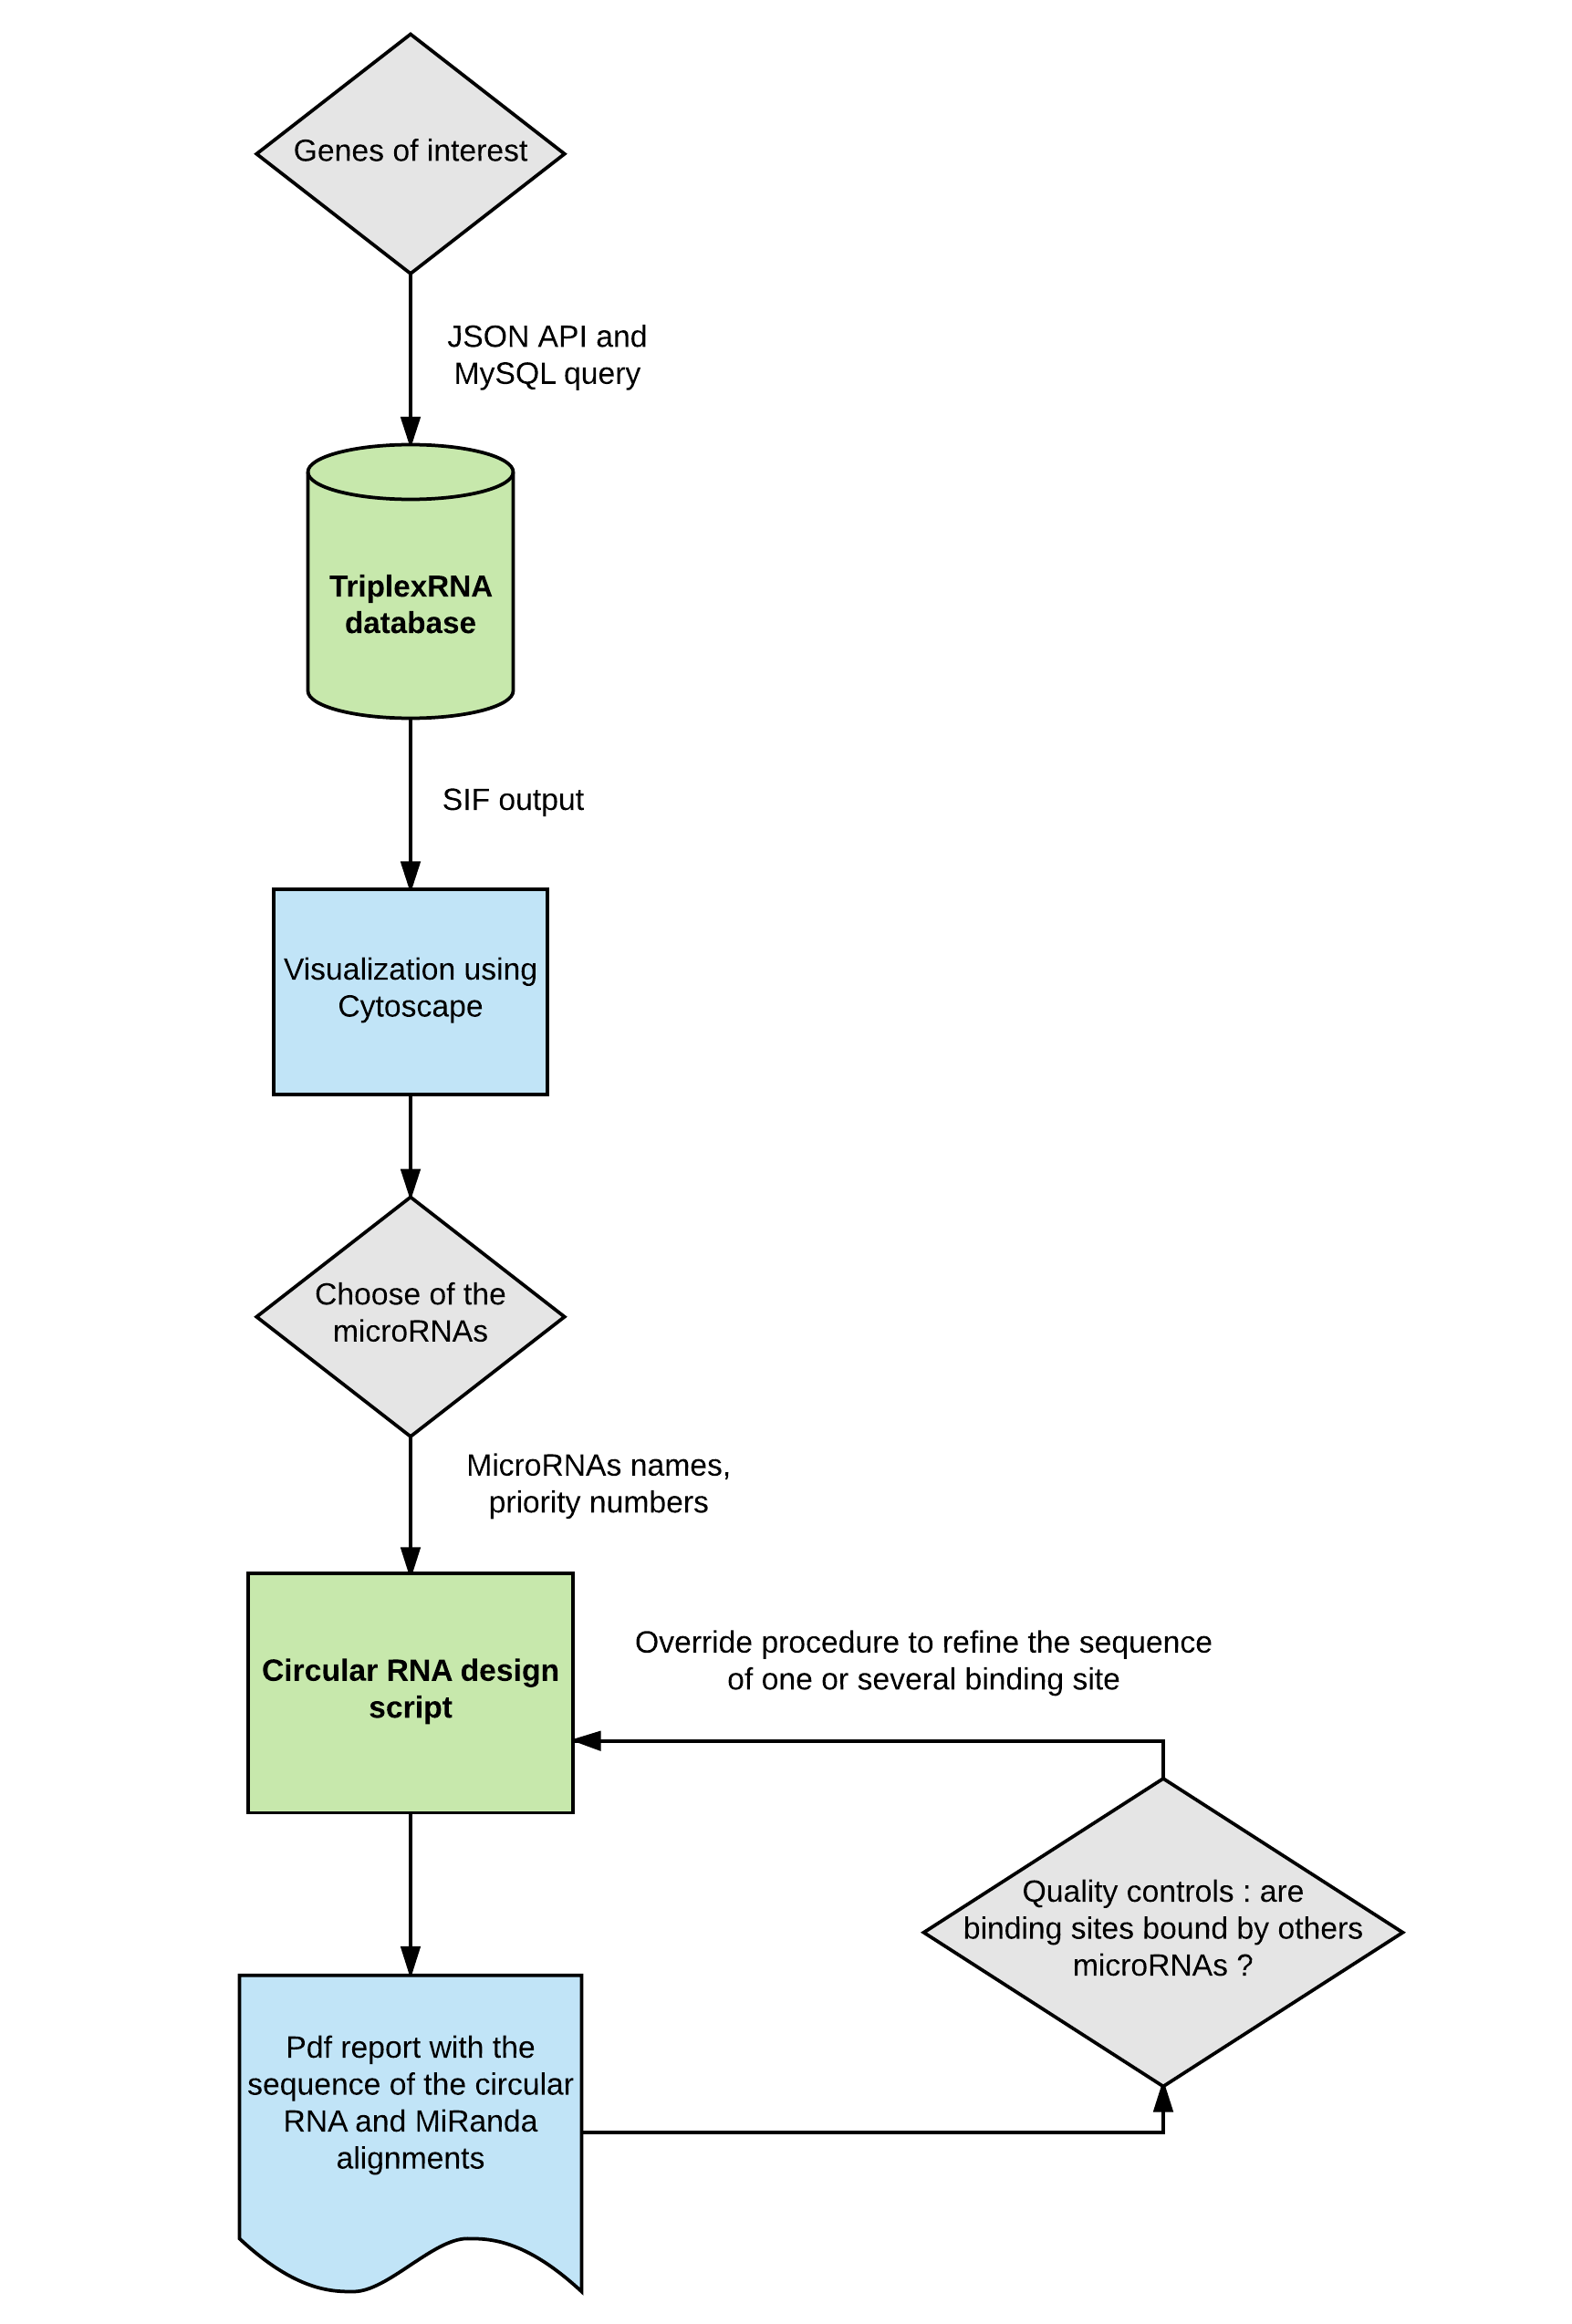
\includegraphics[width=0.9\textwidth]{Final_Workflow.png}}
	\caption{Schematic representation of the final workflow}
\end{figure}

\section{Perspectives}
\subsection{Down-regulation and translational inhibition}


A really important point to keep in mind is that a gene repressed by the microRNAs at the post transcriptional level, in a biological condition of interest, will not necessary appeared as differentially expressed between the biological condition and the control condition after a RNA-seq studies. There is still an ambiguity of whether or not the levels of microRNA-inhibited mRNAs remain unchanged or not \cite{cancer}.\\

In the first case the genes will not appeared as down regulated in a differential, but the transduction of the mRNA will be inhibited and the gene not expressed.\\

A other pertinent approach could be the use of or the integration of miRNA-seq data with the data of the triplexRNA, to investigate directly the microRNAs level of expression.\\
 
More directly, relying on the expertise of the user is another approach and is the form retained for the workflow currently. \\

The user can have - through western blot experiments, for example -, evidences that some genes, while they are not differentially expressed, have the translation of their messenger RNA inhibited.\\

\subsection{KEGGs map}

The differential expression analysis was motivated by the problem of finding which genes are down-regulated or repressed in the biological condition of interest, condition which is the object of the RNA therapy.\\

Indeed, the KEGG pathways are only encode as a list of genes inside the triplex RNA, which does not tell us which gene are down-regulated or which are post-transcriptionaly repressed by microRNAs.\\

A similar information, however, is on the KEGGs map, where the effect of each genes/proteins are indicated. Considering this, an other approach could be to use the KEGGs map to select genes of interest and look at the microRNAs.\\

This is a variation of a feature implemented in the triplexRNA database, which allow a visualization of the mutual target genes for selected microRNA pair, within the KEGG disease pathway. \\

But this feature is for two microRNAs only, and by then ignore the relatives importances of microRNAs among all the pairs, nor it can be done in the direction we would need (a selection of genes downregulated on the map towards all the microRNAs pairs).\\

Anyway, a collection of manually drawn map is not the best material to carry such a task, especially in the optic of a long maintenance.
 
\subsection{Visualization of the triplexes}

In the current workflow, Cytoscape\cite{cytoscape} is used to visualize the pairs of microRNAs which repress the expression of a set of genes.\\

While Cytoscape provide a comfortable way to visualize the pairs of microRNAs, as a software it cannot be part of a pipeline and cannot be integrate directly inside the front-end of the triplexRNA database and require a separate utilization.\\ 

The choice of Cytoscape was done mainly for convenience purpose, and because the author of this document did not find a Python library which would have allow him to fulfill the function of triplexes' visualization. \\

The next step for a core installation inside the triplexRNA of the whole workflow, to enable the creation of the sponge from a web interface should be :

\begin{itemize}
	\item or the development of a visualization tools which can be run in front-end, and which does not require for the user to run a graphical interface by himself separatly
	
	\item or more convenient the use of the headless mode of Cytoscape
	
\end{itemize}


\section{cirMOT1 in hepatocellular carcinoma}

We have seen the example of the circular sponge circMOT1 in the introduction. This circular RNA is correlated with the prognosis of patient of Hepatocellular Carcinoma (HCC) and have been found to promote the expression of p21 by sponging the microRNA mir-9.\\

One thing we can wonder is : does the workflow retrieve mir-9 as a microRNAs to be targeted with a circular RNA in the case of the HCC cancer ?\\

MiR-9 is actually no part of the triplexes involving the CDKN1A messenger RNA. While there is nothing to criticize in the experimental demarche detailed in the article (mir-9 and circMOT1 are clearly identified as responsible for the down expression of p21 and for the inhibition of the repressive effect of Mir-9, respectively), there is several reasons which could explain this :

\begin{itemize}
	
	
\item Among the 99 microRNAs identified using miRanda as susceptible to bind cirMOT1, only 20 of them have been screened for specific enrichment after RNA precipitation in vivo, since they were previously describe as involved in the hepatocellular carcinoma.
	
While this analytic procedure is entirely relevant in the case of a cancer study, for our own problematics of microRNAs combinatorial we are missing the information about the 79 other ones.

Also, while the case of the sponge ciRS-7\cite{mir7} is abundantly cited along the article\cite{carcinoma}, there is no reason to think that most of the natural sponge decoy only one type of microRNA. The supplementals data of Memczak et al,\cite{mir7} are rich in predicted circular RNAs with a seed match for more than one microRNA family. 
	 
\item MiR-9 is over expressed in the hepatocellular carcinoma, and this is why the researcher selected this microRNA for screening after the RNA precipitation. In this situation of over expression, unlike normal conditions, low affinity sites for microRNAs (6-nt sites) become occupied and functional\cite{mir9}. 

Nonetheless, the triplexRNA database has been construct based on binding site predictions extracted from microRNA.org, in which only binding sites with good conservation and good prediction scores were retained\cite{triplex}. This binding sites are assumed to be the ones functional in normal circumstances, with no over-expression of the microRNAs.

That make very likely that the workflow constructing the triplexRNA database does not take into account some microRNAs binding sites which are functional uniquely in some diseases, and by that, it make possible that some triplexes, specifics to particular disease and associated with specific over expression of some microRNAs, are missing in the triplexRNA database.

\end{itemize}

\chapter{Material and Methods}
\startcontents[chapters]
\printmyminitoc %print minitoc


\section{TriplexRNA database}

The TriplexRNA database provide putatives triplexes according to the workflow published here\cite{triplex}, and is available at the following url : https://triplexrna.org/

A triplex is a conformation defined as a messenger RNA and a pair of microRNAs bound on it, in a cooperative manner. 

Two microRNAs are a putative pair of cooperating microRNAs if the seed region of their binding site are separated by a distance of 13-35 nt \cite{coop}

A triplex is supposed functional - meaning : the pair of cooperative microRNAs exert a corepression - if the triplex adopt a conformation called "canonical triplex", discribing a conformation where the two microRNAs bound the messenger RNA without overlap or mutual exclusion, with a preservation of the seed binding for both of the microRNAs.

\begin{figure}[H]
	\centering
	{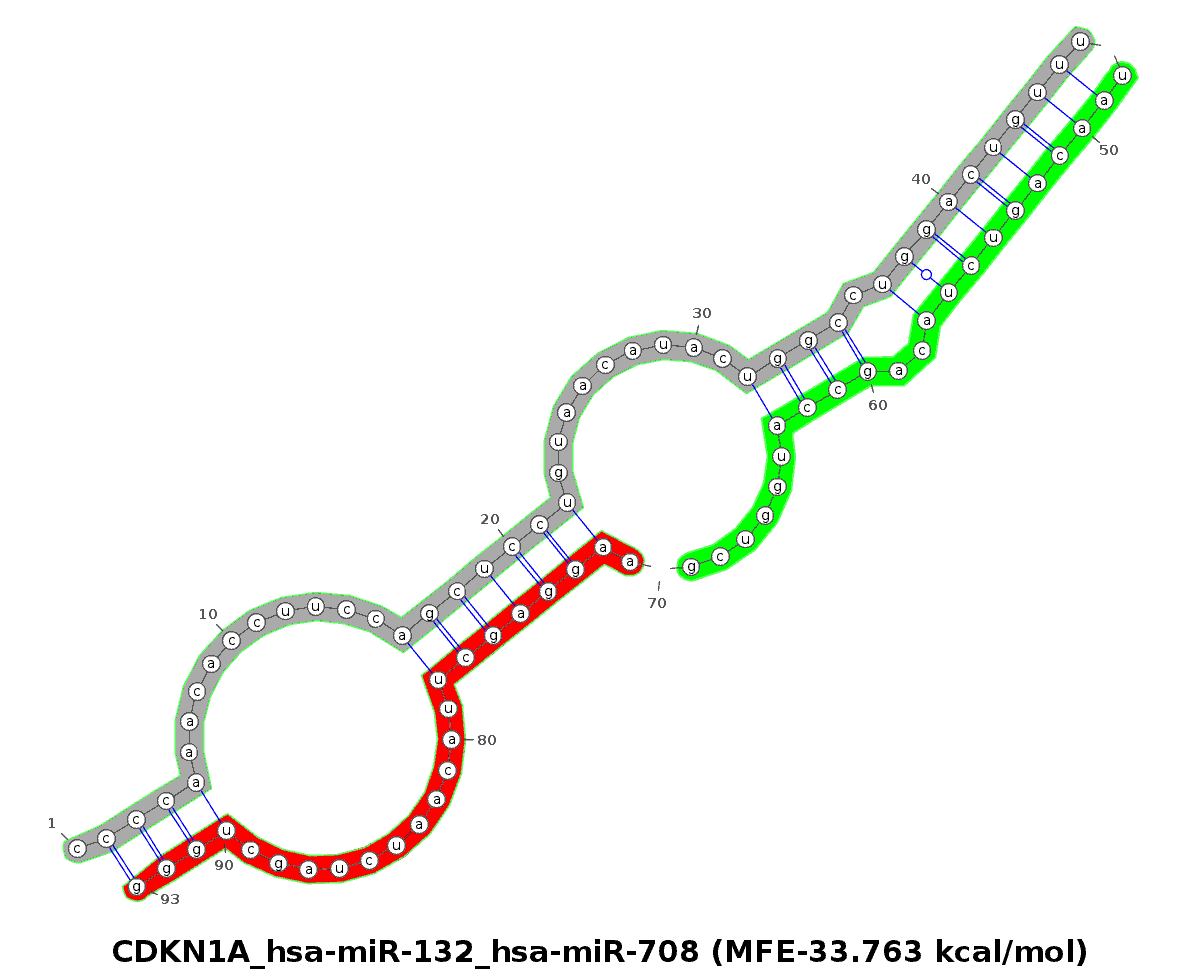
\includegraphics[width=0.5\textwidth]{canonical.png}}
	\caption{An example of canonical triplex, from the triplexRNA database}
\end{figure}

The triplex database can be interrogate through the web instance, using a JSON query. The database is also composed by three SQL table :

\begin{itemize}
	\item A table listing the triplexes for their cognate genes in the mouse. 
	\item A table listing the triplexes for their cognate genes in the human.
	\item A table associating genes and their cognate triplexes with a Kyoto Encyclopedia of Genes and Genomes (KEGG) pathways identifier (ID)\cite{KEGG}.
\end{itemize}

Each of them can be query using MySQL.
The triplexRNA database which is interrogate with a MySQL request in the script Query Triplex is a local instance, different from the web instance called by the JSON queries (but both contains the same data).

\section{Request of triplexes and gene inside the Melanoma Pathways}

The list of the genes inside the KEGG Melanoma pathway\cite{KEGG} was retrieved by querying the corresponding SQL table for all the genes associated with the KEGG ID of the pathways (hsa05218).

The triplexes for this list of genes was then retrieved using the JSON query for a list of genes, as describe below.

\section{SIF format, output of the JSON query}

The sif format is the input format used for visualization using cytoscape \cite{cytoscape}. 

This format specifies only nodes and interactions and it is written as follow :
\\

nodeA relationship\_type nodeB \\
nodeC relationship\_type nodeA \\
nodeD relationship\_type nodeE nodeF \\
Which, for the purpose of visualizating the microRNAs involved in the most triplexes, became, as outputted by the executable which retrieve all the triplexes for a list of genes :

microRNAname ID\_of\_the\_triplexes microRNA2name

\section{JSON query of a list of genes}

The script which retrieve the functionnal triplexes take as input the name of a txt file containing the list of genes.

This list is then used to query the triplexRNA database with a JSON query and keep only the functionnal triplexes for each gene. The JSON query retrieve data under the form of JSON dictionnary that the script can then parse. Here an example of JSON query to retrieve all the triplexes associated with CDKN1A :

\lstinputlisting{json.py}

The script also filter the triplexes considered as redundant. The output is wrotte in a sif format, in a separate folder, with a global report.

\section{Filtering of the redondant triplexes}

The redundant triplexes are filtered out considering the following : if a triplex in the list of triplexes associated to a gene has : 
\begin{itemize}
	\item the same position of beginning or ending for the microRNA's binding position of one already retained microRNA, for the first microRNA composing the triplex
	\item or the same position of beginning or ending for the microRNA's binding for the second microRNA composing the triplex, 
	\item and a name of one microRNA in common with a triplex already retain for the sif output of this gene;
\end{itemize}

Then this triplex is considered as redundant and ignored for the sif output.
The triplexRNA database which is interrogated with the MySQL request for the filtering is a local instance, different from the web instance which is the one queried with the JSON request. 

\section{Genes level of expression, Melanoma cancer}

The level of gene expression for the Melanoma cancer used for the differential expression are RNA-seq data, published by the The Cancer Genome Atlas Network (TGCA) \cite{TGCA}, from the project TGCA - Melanoma (SKCM).

The gene expression profiles was measured experimentally using the Illumina HiSeq 2000 RNA Sequencing platform by the University of North Carolina TCGA genome characterization center. This data are level 3 data, meaning that the gene-level transcription estimates are in log2( transformed RSEM normalized count + 1), and have been produced from a cohort of 331 patient \cite{TGCA}.

The level of expression for the genes composing the KEGG melanoma pathways have been download through the Xena browser (http://xena.ucsc.edu/) \cite{Xena}. UCSC's Xena is a data server-based platform that contain functional genomics data and output them in response to request done through a web graphical interface. 

The Xena browser was used to retrieve the level of gene expression for each sample, associated with a phenotype [pathologic\_stage], the categories of phenotypes going from the stage 0 to IV. This indices describe the extent of the cancer. See the pdf from the american joint committee on cancer \cite{joint}


\begin{figure}[H]
	\centering
	{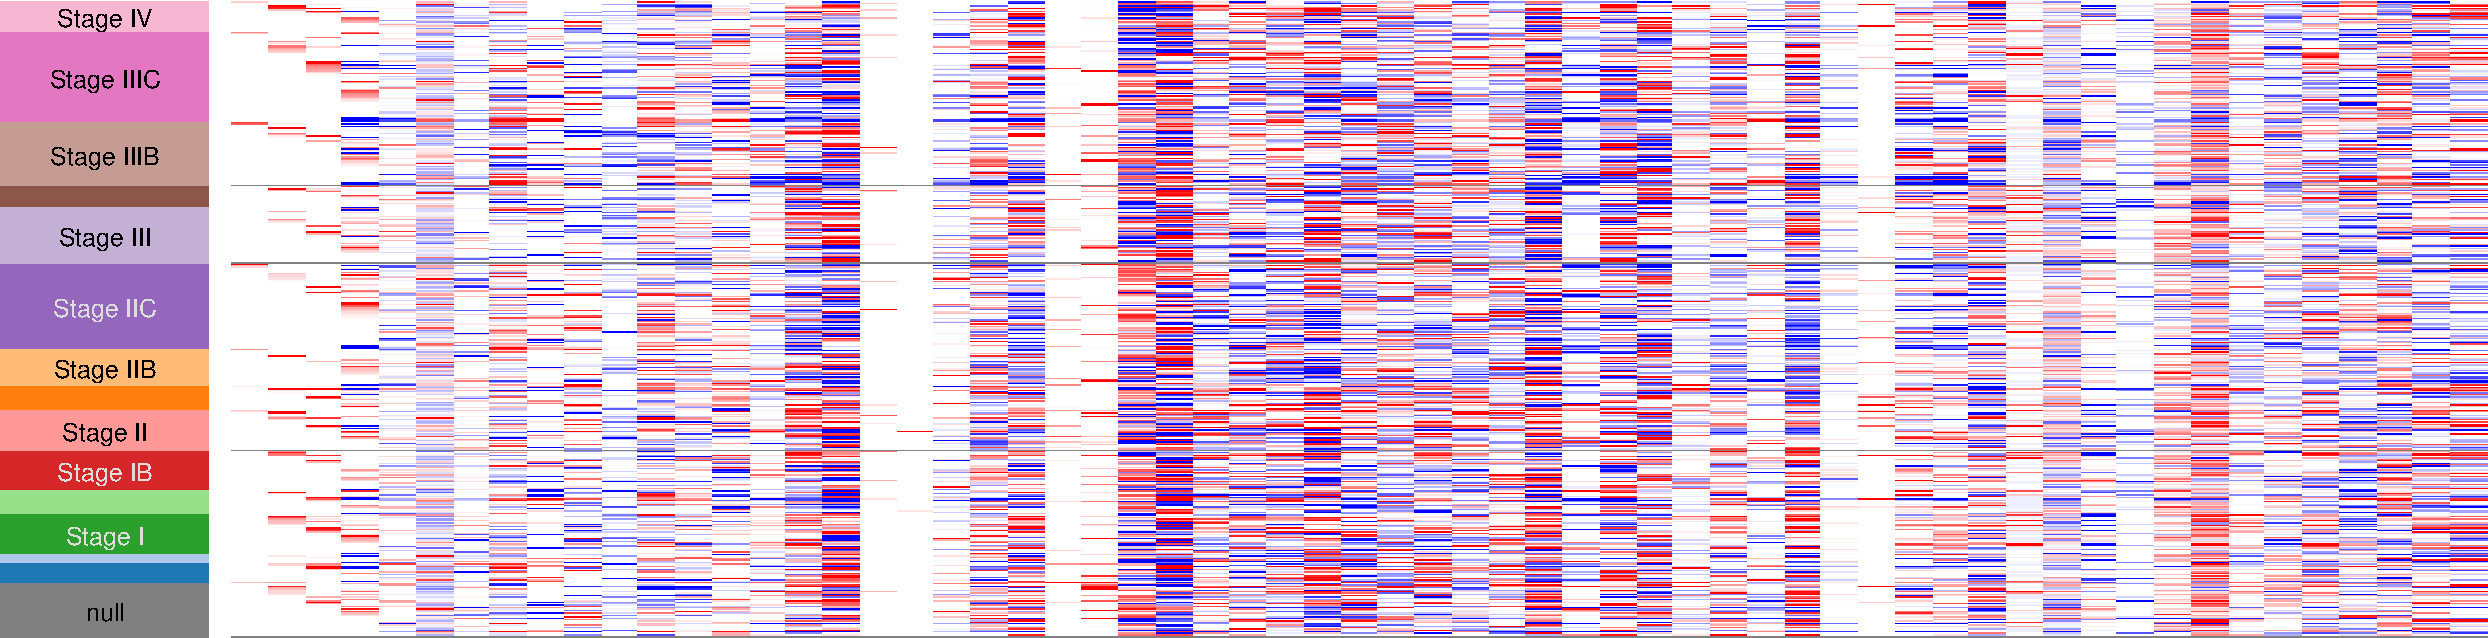
\includegraphics[width=1\textwidth]{Xena_melanoma.pdf}}
	\caption{Web visualization of the level of gene expression, associated with the phenotype [pathalogic\_stage]. This levels of expression can be then download.}
\end{figure}

\section{Colorectal cancer data}

The level of genes expression for the colorectal cancer was extracted from the R package curatedCRCData \cite{curated}, a package providing manually curated data of microarray and RNA-seq data from the TCGA-COAD project.

The level of gene expression are RNA-seq level 3 data, in log2 ( transformed RSEM normalized count + 1), the same format than the RNA - seq data of the TGCA - SKCM project.

\section{Graphical visualization of the cooperation between \\ microRNAs}

The  visualization of the cooperation between microRNAs in a form of graph has been done using Cytoscape\cite{cytoscape}, an open source software for integrating biomolecular interaction networks.

The format used as input to construct the network is the .sif format, cf the SIF format section above.


\section{Differential expression analysis for melanoma and colorectal cancer data}

The differential genes expression analysis between early and late melamoma stage has been done using gene-level transcription estimates in log2(x+1) transformed RSEM normalized count, provide by the TGCA-SKCM project, using the Limma package in R \cite{limma}.

After Quantile normalization to equalize the library sizes\cite{limma}, Limma has been used to fit a linear model to the already log 2 - transformed data using an empirical Bayes method\cite{limma}.

The same procedure has been employed for the colorectal cancer data.


\section{Randomized Lasso}

The randomized lasso has been used  on the gene-level transcription estimates in log2(x+1) transformed RSEM normalized count, provide by the TGCA in the project SKCM, using the python scikit-learn library\cite{scikit}.

\section{Random Forest}

The Random Forests has been trained using 2500 tree, 0 random state, directly on the gene-level transcription estimates in log2(x+1) transformed RSEM normalized count provide by the TGCA in the project SKCM, using the python scikit-learn library \cite{scikit}.
The testing set of data has been generate by selecting at random 20 percent of the total data set.

\section{Random Forest Classification Error Plotting}

The plotting of the error of the Random Forest has been done using the python library forestci. 

\section{Minimum Free Energy Calculation and Vizualization}

The Minimum Free Energy Calculation is performed using the tool RNAfold of the package ViennaRNA 2.3.5. \cite{vienna}

\section{MicroRNAs alignments}

The circular design script is provided with a copy of the mature.fa file from the last release of mirbase, downloaded in may2017, containing all the mature microRNAs referenced in the database. 

An alignement using miRanda \cite{Miranda} is performed for each cluster against every human microRNAs, with the options "-noenergy -strict -sc 150". This options restrict the alignements to the ones with a strict alignment in the seed region (positions 2-8) region and eliminate results with little to no biological sense.

\section{Pdf report}

The pdf report is created using the web tool TEXPILE, developed by Martin Scharm. TEXPILE is a web service design to be an online compiler for LaTeX projects. The report is first write in the Tex language by the circular RNA design script. This Tex file is then convert into a pdf file by the TEXPILE tool.

TEXPILE's code is hosted at GitHub: github.com/binfalse/TEXPILE



\bibliography{bib.bib}

\end{document}  
